%!TEX encoding = UTF-8 Unicode
%!TEX TS-program = xelatex
%% This template licensed under CC-BY-NC-SA by Koenraad De Smedt
\documentclass[letterpaper,12pt]{article}
\usepackage[margin=1in]{geometry}
\usepackage{graphicx}
\usepackage{setspace}
\onehalfspacing

% \usepackage{fontspec,xltxtra,polyglossia,titling,graphicx}
% \usepackage{verbatim,gb4e,synttree,multicol} % choose or add what you need
\usepackage[colorlinks,urlcolor=blue,citecolor=blue,linkcolor=blue]{hyperref}
%\setmainfont[Mapping=tex-text]{Times New Roman} % or another similar font
%\setdefaultlanguage{english}

\usepackage{subcaption}
\usepackage{fancyvrb}
\usepackage{natbib}
\usepackage{tabularx}
\bibliographystyle{abbrv}

\title{Real-Time 3D Reconstruction from ROV Camera Arrays of Opportunity}

\begin{document}
\begin{center} 
\thispagestyle{empty}

\vfill

{\large NOAA Office of Exploration and Research (OER)\\
Award \#NA160AR0110195}

\vspace{1em}

\textbf{\Large Real-Time 3D Reconstruction from ROV Camera Arrays of Opportunity}

\vfill

PI: Aaron Marburg \\
University of Washington  \\
Applied Physics Laboratory \\
Seattle, WA \\
amarburg@apl.washington.edu \\
206-685-8461

\vfill

Funding:  \$105,720 \\
Period of Performance:  9/1/2016 -- 8/30/2018\\
Progress Report for Period:   9/1/2016 -- 8/30/2018 \\
\textbf{Final Report}

\vfill 

%
\end{center} \clearpage
\pagenumbering{arabic}


\subsection*{Abstract} 

This project examines the use of photogrammetric 3D reconstruction to build 3D models (point clouds) of scenes observed by the ROV Deep Discoverer (D2) using exclusively the HD main science camera video collected as part of normal ROV operation.   To this end, the project works with archival video from two dives (out of four dives provided by NOAA OER) from expedition \textit{EX1605: Deepwater Exploration of the Marianas} to attempt 3D reconstruction using frames drawn from short segments of each dive.   Reconstruction was attempted with two software tools: Agisoft Photoscan, a commercial, post-processed reconstruction package which has proven to be robust to a diversity of input data types, and a heavily modified version of the open source real-time reconstruction package LSD-SLAM (Large Scale Direct Simultaneous Localization and Mapping).   Photoscan successfully produced 3D models from sets of images drawn from short (5-10 minutes) segments of video, constrained primarily by the duration of the ROV's residency at each site.    As a post-processed tool, each reconstruction required between 2 and 4 hours of processing, not including time to extract the scene of interest within the ROV video.  In contrast to Photoscan, LSD-SLAM is designed for realtime ``online'' processing, building and expanding the 3D model incrementally as new data comes in from the camera.    Realtime processing brings two significant advantages:   first, it provides immediate feedback on the quality and coverage of reconstruction while the ROV is in the water.   This could lead to, for example, a decision to allocate additional time to capturing particular details of a site to ensure the quality of a later post-processed reconstruction   Second, the 3D model generated through realtime reconstruction provides situational awareness of the ROV's position relative to the local environment, which can assist with further mission planning.    Despite intensive development to improve the robustness, maintainability and performance of LSD-SLAM, the package was not able to complete a reconstruction of the selected video segments. 

\section{Summary}

\subsection{Purpose of Project}

This project examined the applicability of photogrammetric 3D reconstruction to ROV-based deep-ocean exploration.   Photogrammetric or image-based 3D reconstruction is the process of using large numbers of still images (or frames from video) to produce a 3D model of the scene shown in the images.   In its simplest form, photogrammetric reconstruction requires only a sequence of images as an input, estimating both the scene's 3D structure and the camera positions through a non-linear optimization.   To form this optimization, the reconstruction uses image-patch-matching techniques to find points in two or more input images which correspond to the same world point, with each of these inter-image correspondences forming a geometric constraint.   Given sufficient numbers of these constraints, a bulk non-linear optimization, typically referred to as \textit{bundle adjustment}, can be solved for both the 3D arrangement of the world points and for the camera positions.  Having established the camera positions, a stereo-matching algorithm can be used to then fill in the point cloud between the previously extracted world points.  The general field of reconstruction tools can then be further divided into post-processed and real-time operations.   The former focuses on reconstruction from sets of images after collection.  As such, the sets of images are often hand-selected or hand-curated from a larger original data set; processing time or performance is less of a concern; and the processing does not necessarily know or take advantage of the order in which images are taken.   As the reconstruction software has access to the full sequence of images, it actively seeks image correspondences across all pairs to form a dense network of constraints, and can generally be considered ``optimal'' for a given set of input images.   However, post-processed results may take hours or days to produce and are not generally available for review while data is being collected.

Alternatively, real-time reconstruction algorithms are designed for processing data as it streams in, either as video or a sequence of images.   In contrast to post-processing, real-time algorithms are heavily tuned for performance and in many cases sacrifice the resolution, if not the accuracy, of the resulting reconstruction to process incoming data in a timely manner.   Real-time algorithms also privilege matches between the current image and recent images over more temporally distant images, and as a broad generalization produce less complete inter-image correspondence sets and thus less optimal final products.   In exchange for this reduced data quality, real-time algorithms offer the possibility of ``growing'' a 3D reconstruction incrementally as new data arrives from the sensor, allowing immediate review of reconstruction quality.    From a data point of view, this immediate feedback might be used to identify and remedy data quality issues which might impact later post-processed reconstructions.  For example, a real-time reconstruction would show regions in a scene which had not yet been imaged as ``holes'' or data voids, which could then be explicitly filled as part of the ongoing data collection.   With the long processing cycle of post-processed reconstruction, this data gap might not be noticed until after it is too late to remedy.  In the future,  live reconstruction could also play a part in on-line mission planning and visualization, for example, providing a 3D map of a vehicle's trajectory and current location within a scene.  This could assist in scene-relative navigation (e.g., ``return to that object which is behind you and to the left'').    Taking an even longer view, scene information from 3D reconstructions can be used as an input to robotic algorithms for autonomous or semi-autonomous mapping and exploration by unmanned underwater vehicles.  

As high-quality imaging data is relatively simple to acquire, photogrammetric reconstruction has become a popular technology for ``3D scanning'' of objects and scenes.  However, due to its computational complexity and sensitivity to certain conditions in image acquisition, it has excelled in certain niches (large scale outdoor acquisition, particularly from small aircraft/``drones'') whereas other, more specialized technologies (e.g., structured light sensors, LiDAR) are more prevalent in other applications.      Due to the challenges in developing and adapting new technologies for subsea use, the ability to exploit the broadly installed base of video cameras on ROVs becomes even more attractive.

\subsubsection{Describe and list the project objectives}

The broad question addressed here is the applicability and utility of 3D reconstruction to ROV-based exploration, and particularly as a value-added product when it was not an explicit mission goal.  This project, then, addresses three main questions:

\begin{itemize}
    \item First, are segments from the provided ROV video suitable for post-processed 3D reconstruction?   Are there structural or operational impediments to performing 3D reconstruction with this video?   Post-processed reconstruction may be a valuable added product from particular ROV dives, particularly when exploring sites where the geometry of the site at a $\sim 1-10$ m scale is of particular interest.  As reflected in the dive segments analyzed within this project, this includes many archaeological explorations,  hydrothermal vent structures, and larger coral reef communities.   As shown in one of the dives (EX1605L3\_DIVE04), reconstruction can also be useful for visualizing topography over short transects.
    
    \item Second, having shown that a segment of video can be reconstructed under controlled post-processing conditions, can those same segments be reconstructed using a real-time algorithm?   This question occupies the bulk of this project for two reasons:  first, as discussed previously, real-time reconstruction is inherently a technically more challenging endeavour than post-processed reconstruction.  Second, whereas the post-processed reconstruction uses a commercial off-the-shelf software tool, there are no commercial real-time reconstruction software packages.  Instead, most real-time software remains in the academic realm, and requires significant effort to understand, use, and modify for specific applications.  

    \item Finally, having processed video from a variety of missions, is it possible to make a general statement about the suitability of the collected video for 3D reconstruction?  This is a multi-faceted question.  First, is the video data itself suitable for reconstruction?  Given the overall image quality of the main HD camera, this is assumed to be true.  Second, do the procedures for recording and storing archival ROV video enable reconstruction?   Finally, and most importantly, are the standard operating procedures for the ROV \& camera amenable to reconstruction when reconstruction is not the explicit mission goal for a dive or segment of a dive.  During a dive, the ROV and camera motion are driven by a large number of stakeholder needs and constraints, ranging from the capabilities and physical safety of the ROV, through to the science goals of the staff onboard the \textit{Okeanos Explorer} and on telepresence.  In an ideal world, reconstructions could be produced without significant additions to this set of constraints; or as a compromise, through a well-defined set of standard operating procedures for collecting data for reconstruction.  
    
\end{itemize}

% \subsubsection*{Describe issue that was addressed}


\subsection{Approach}
\subsubsection{Describe the work that was performed}

Project development fell into three major tasks.  First was acquisition of the archival D2 video and development of tools for accessing and extracting useful subsets of the video.  This development also included exploration of the ~32 hours of supplied video to identify short segments suitable for reconstruction.   Second was the processing of those subsets using Agisoft Photoscan, a commercial 3D reconstruction package.   Third was the processing of those same subsets using LSD-SLAM, an open-source realtime reconstruction tool.  Whereas Photoscan could be used out-of-the-box for the second task, the third required significant development of the LSD-SLAM code base to produce a robust realtime reconstruction solution.  

Input video was provided from the NOAA data archive.  In collaboration with archivists, four dives from NOAA expedition \textit{EX1605: Deepwater Exploration of the Marianas} were identified as having regions which might of interest when reconstructed:

\begin{itemize}
    \item \textbf{Leg 1, Dive 11: New Vent Field} (\textit{EX1605L1\_DIVE11}).   An approx 6h30m dive exploring an area previously mapped by the Sentry AUV and believed to contain multiple previously unexplored hydrothermal vents. This dive was selected as hydrothermal vent structures provide a dramatic 3D shape which might be explored in more detail through reconstruction.    This video would be challenging due to the high level of motion around a vent due to thermally-induced schlieren, macrofauna, and particulates/precipitates/smoke.
    
    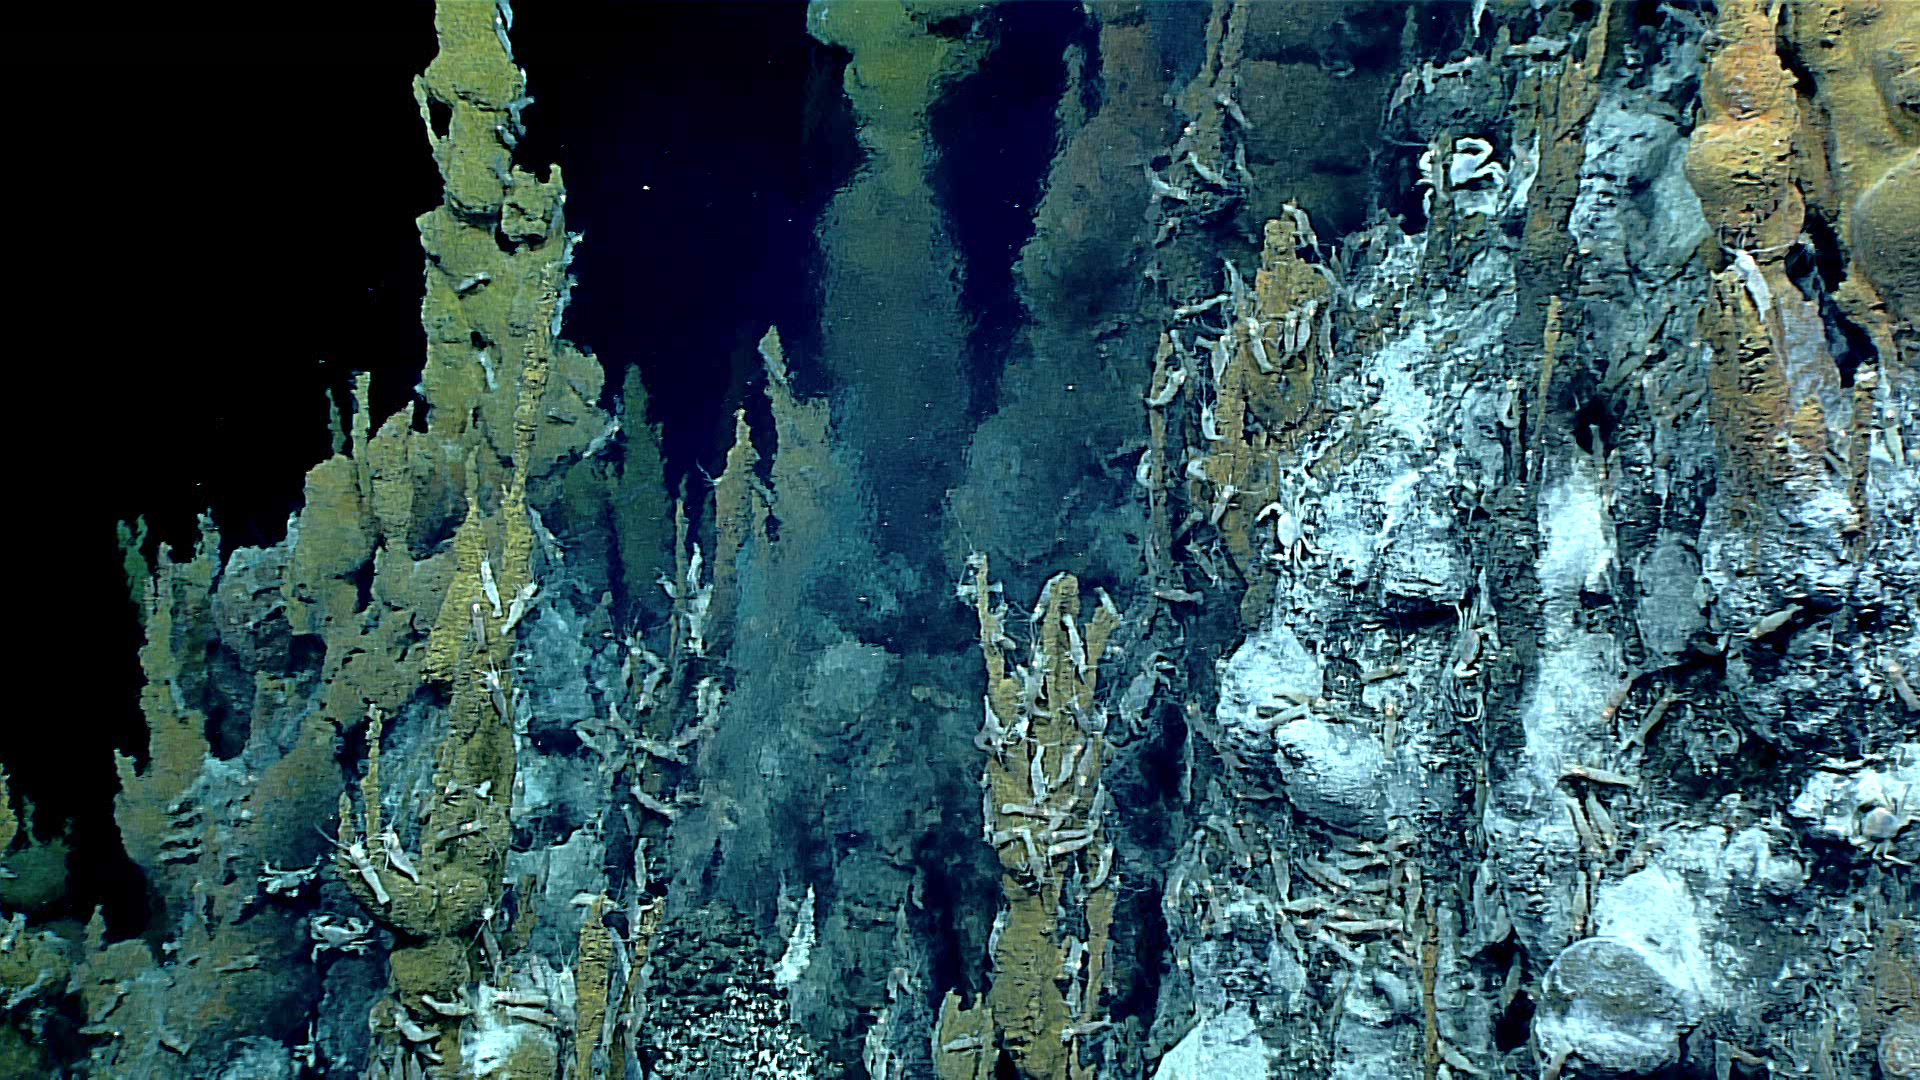
\includegraphics[width=0.5\textwidth]{images/EX1605L1_DIVE11_highlight.jpg}
    
    \item \textbf{Leg 3, Dive 4: Hadal Ridge} (\textit{EX1605L3\_DIVE4}).  Approximately 2h51m of this 10h dive was spent on the bottom, transecting up-slope across a region of fine sediment with some rocky outcroppings.  This video was selected to evaluate the potential of using photogrammetry to estimate vehicle trajectory during long transects.
    
    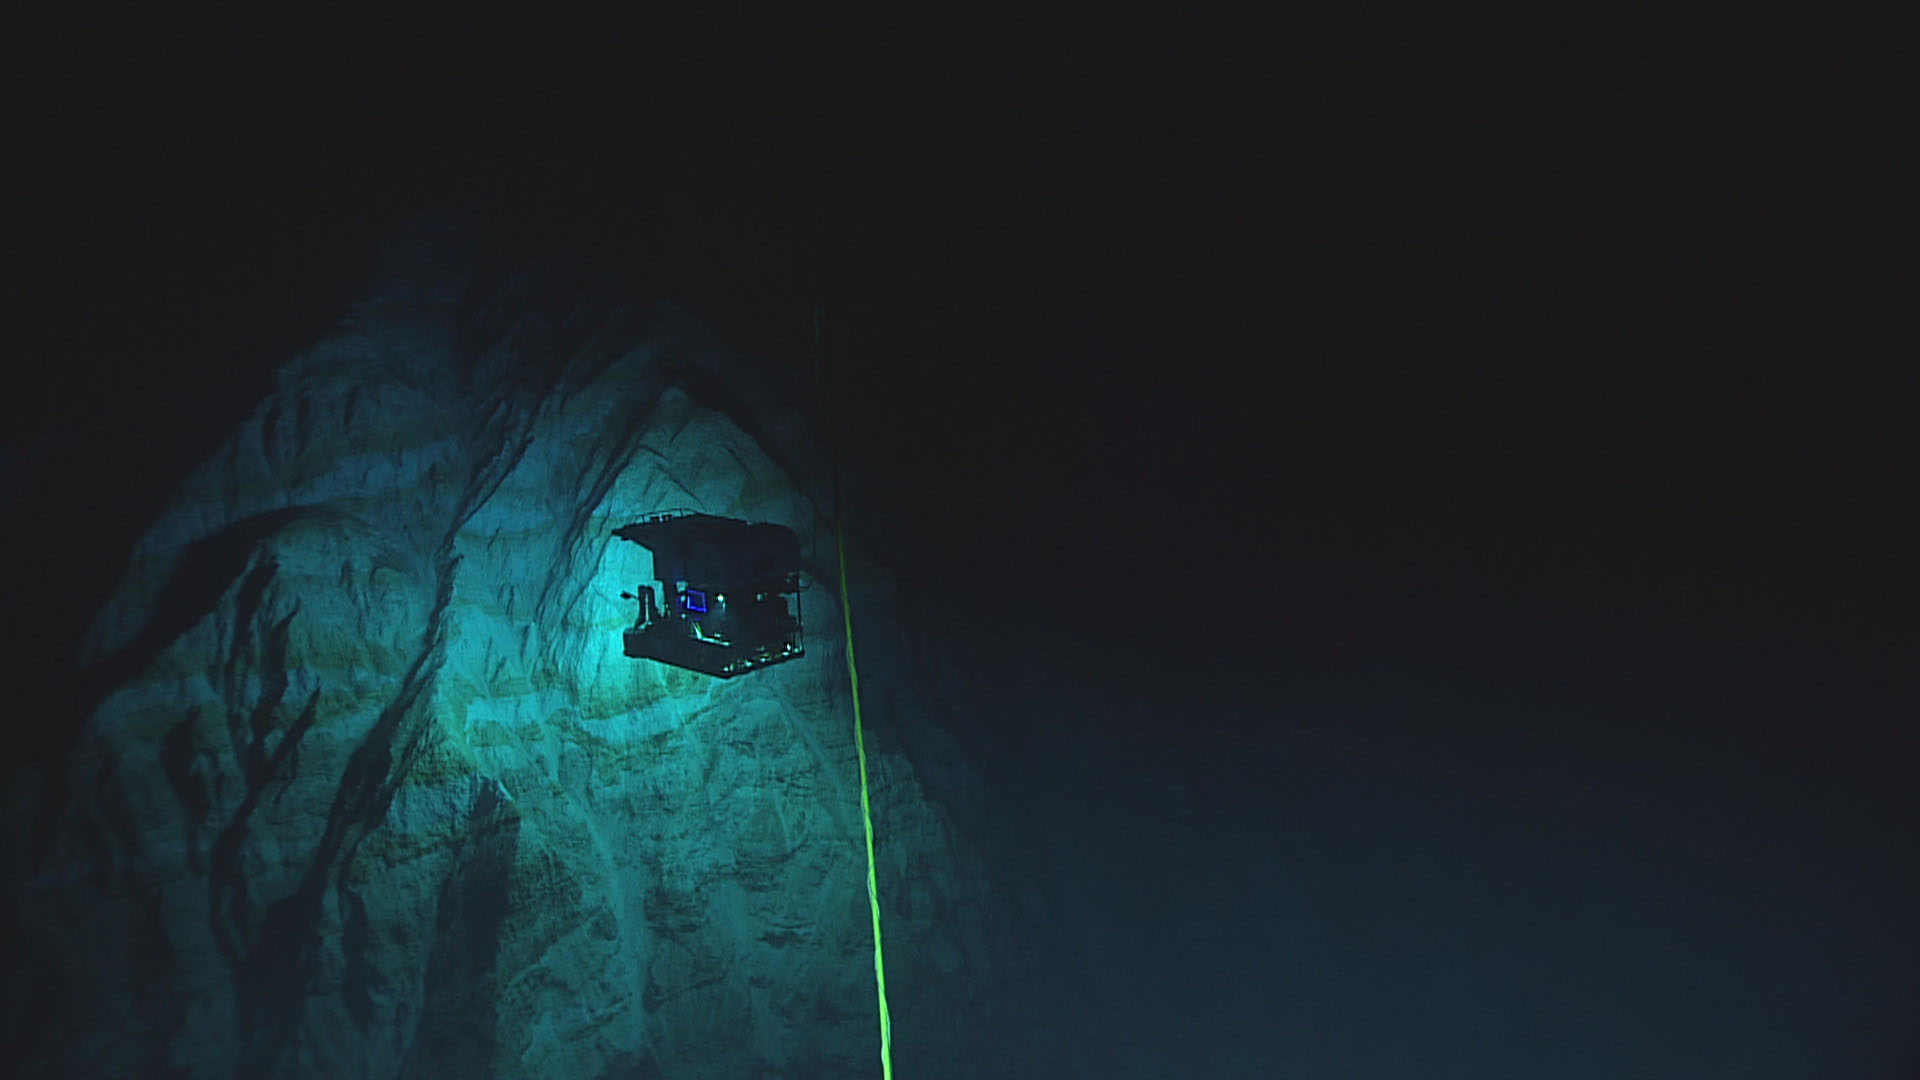
\includegraphics[width=0.5\textwidth]{images/EX1605L3_DIVE4_highlight.jpg}
    
    \item \textbf{Leg 3, Dive 7: Chamorro Seamount} (\textit{EX1605L3\_DIVE7}).  Approximately 7h on the bottom in a rocky region including several smaller hydrothermal vents.    This video was selected to evaluate reconstruction of smaller rocker outcropping and vents, and also for mapping of transects over rocky terrain.
    
    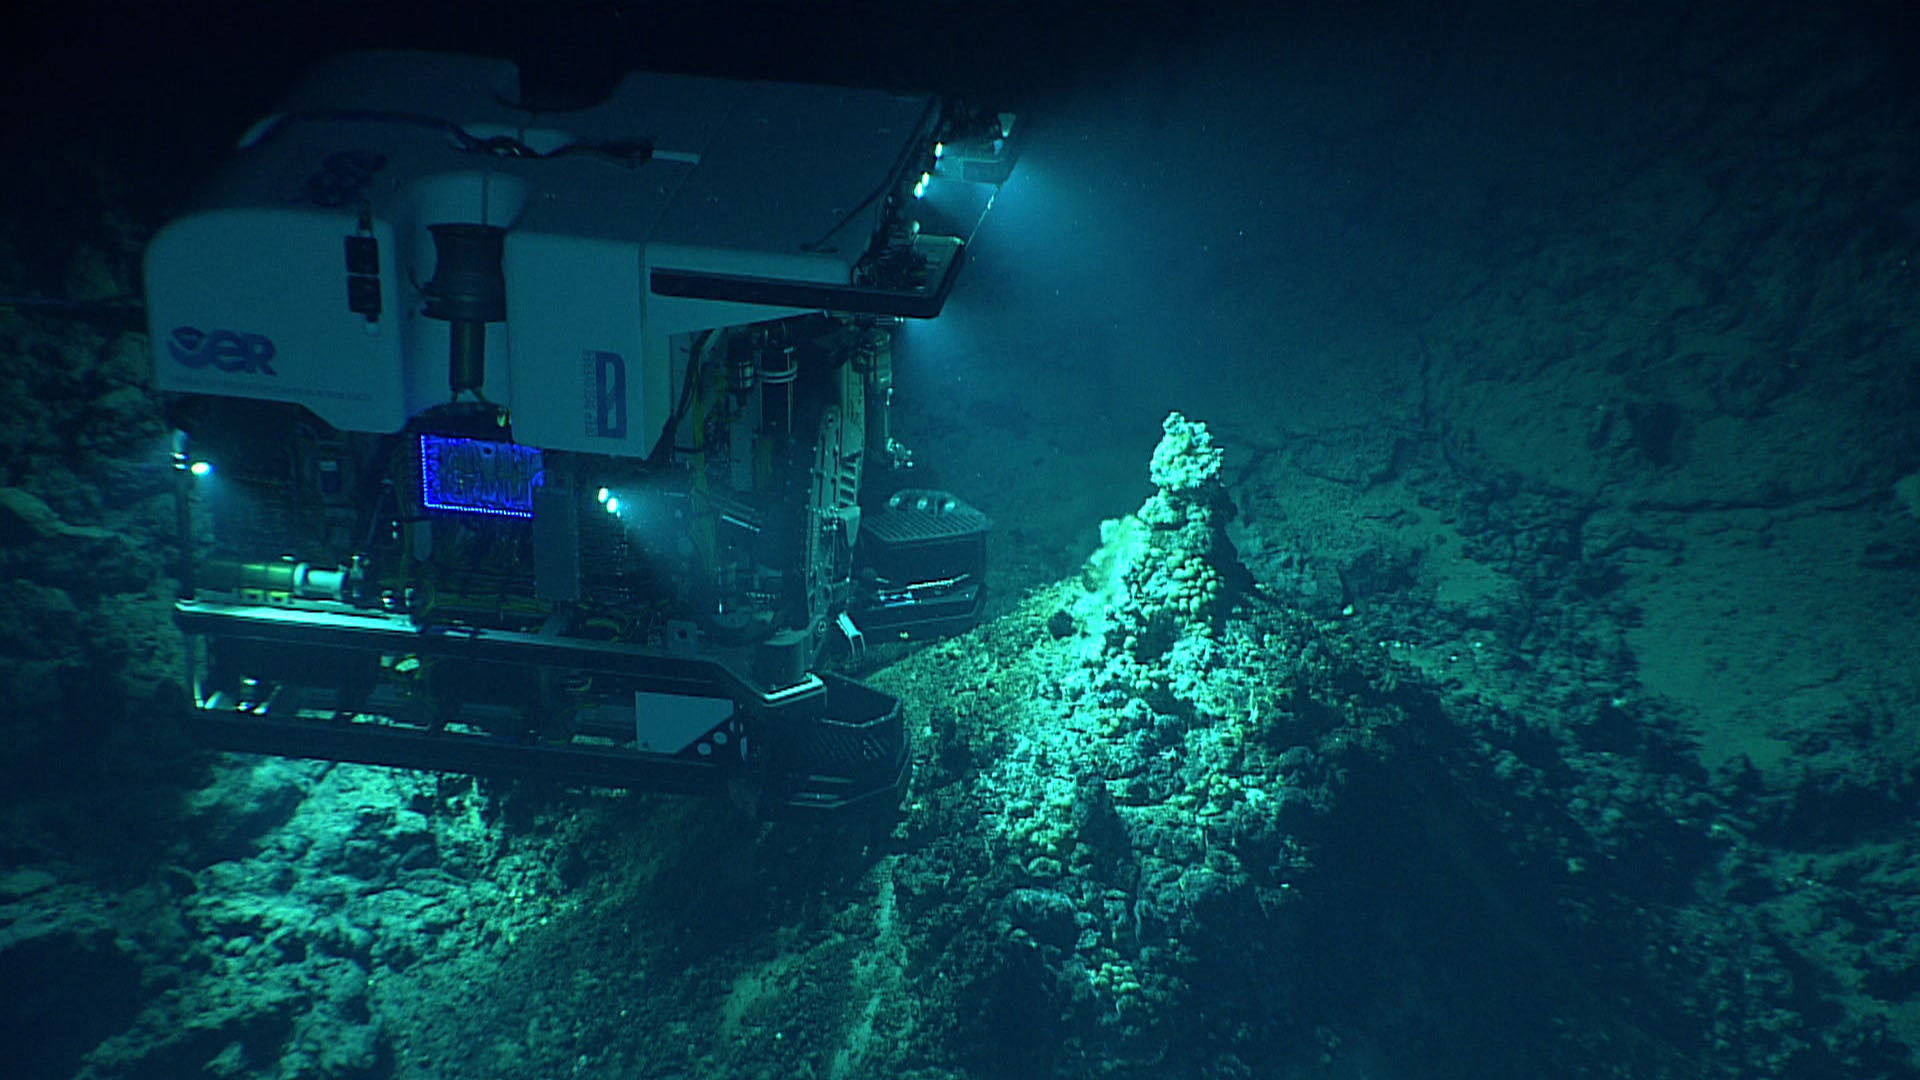
\includegraphics[width=0.5\textwidth]{images/EX1605L3_DIVE7_highlight.jpg}
    
    \item \textbf{Leg 3, Dive 22: Romeo and Juliet} (\textit{EX1605L3\_DIVE22}).  This dive explores two sonar anomalies in the Saipan channel believed to be wreckage of B-29 aircraft from World War Two.  This video was selected to demonstrate reconstruction of archaeological sites.
    
    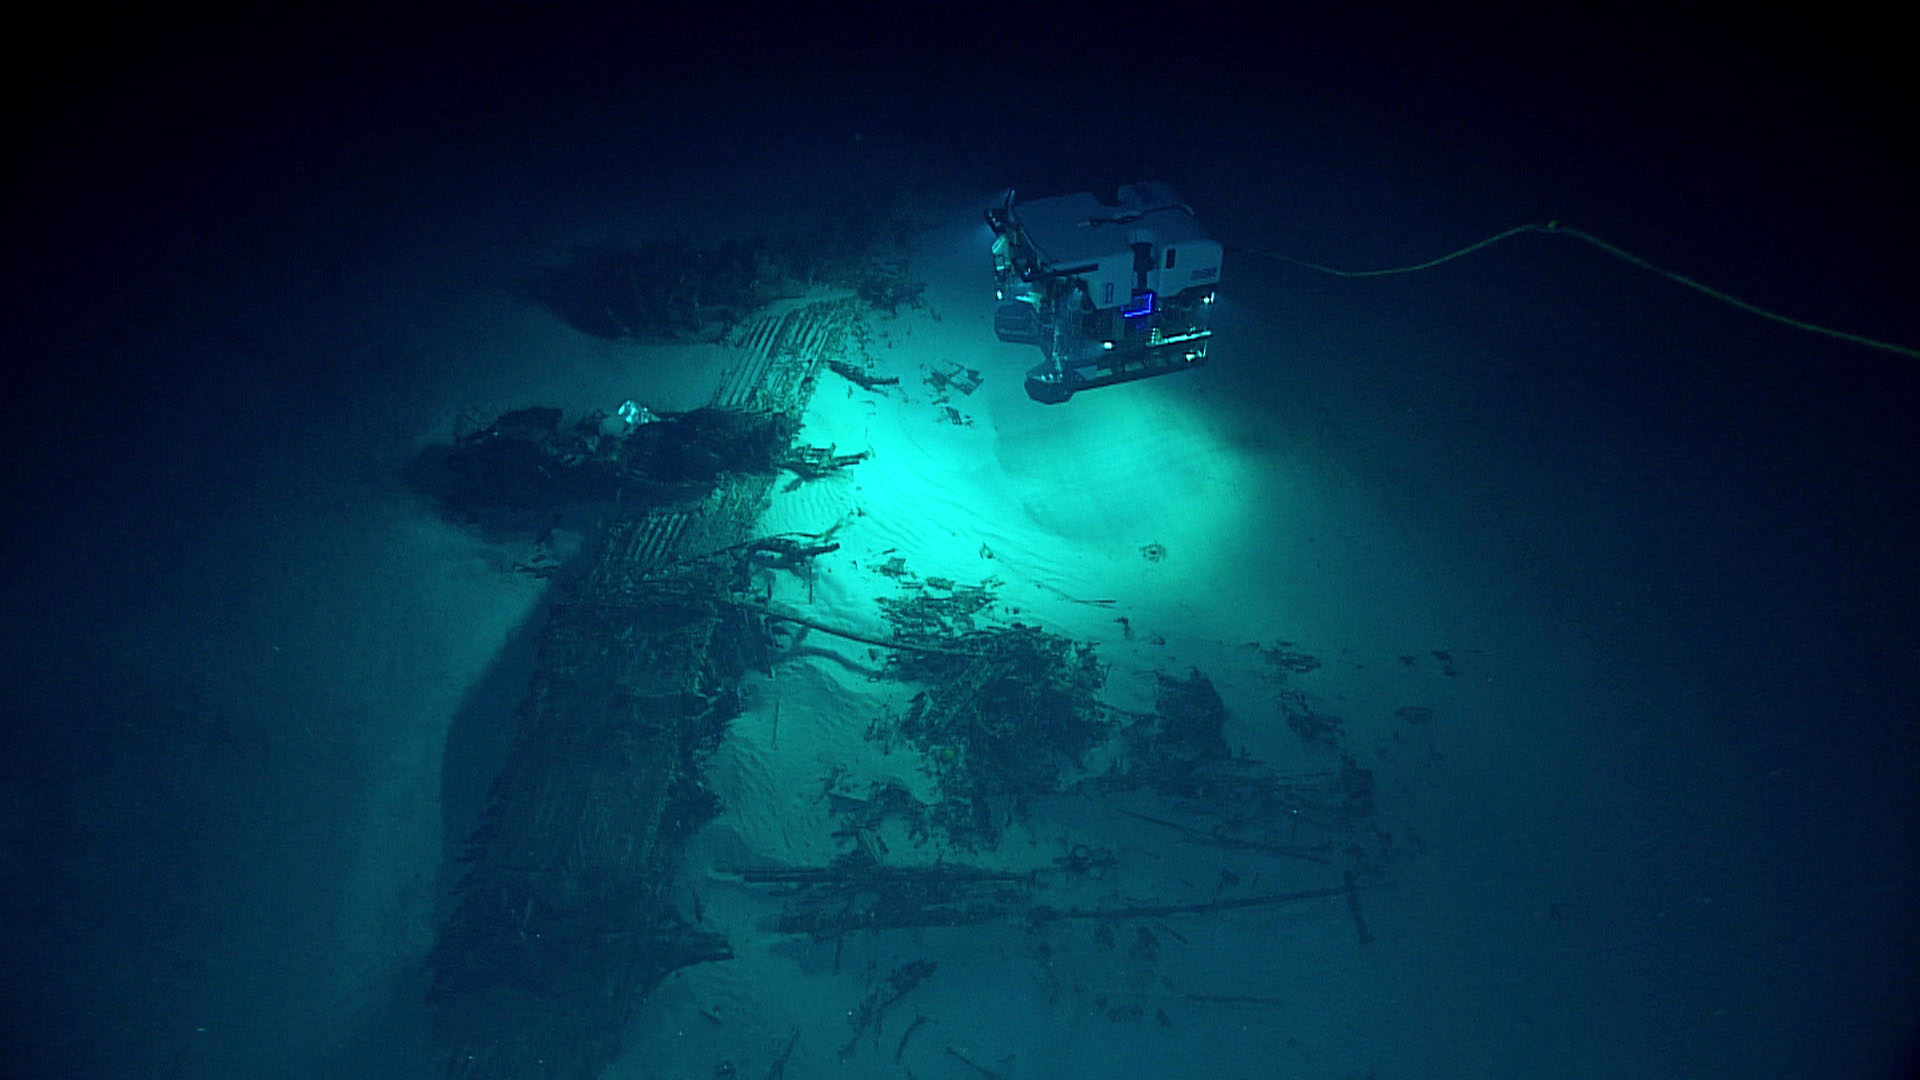
\includegraphics[width=0.5\textwidth]{images/EX1605L3_DIVE22_highlight.jpg}
    
\end{itemize}

\noindent
Approx 4.2TB of video was delivered by external hard drive from the NOAA data archive.  Multiple video products for all four dives were provided, including the full HD-resolution QuickTime/ProRes-encoded stream from the main science camera, as well as selected video subsets from both the main science camera and supplemental cameras, including the brow cameras on D2, and the \textit{Seirios} camera.   The latter supplemental data sets were not continuous through the dive and were provided at each camera's resolution, typically standard definition (SD).  

\subsubsection*{Describe how the project was organized and managed}

All project work was performed and managed by the PI at UW-APL.

\subsubsection*{Describe how data was organized, processed, and archived}

The science camera video was provided by NOAA as sets of video files spanning each of the four dives of interest, from descent through ascent.   The files are split into 5 minute segments, and total approximately 4.2 TB for all four dives.   Data was delivered via an external hard drive and was subsequently stored in its original directory structure on a network drive at UW-APL.  Every effort was made to maintain the original data in its original format rather than perform extensive reorganization of the original raw video data.

\subsection{Findings}
%\subsubsection*{Describe actual accomplishments and findings}

\subsubsection{Video Indexing and Annotation}

Initial work focused on the full-resolution, full-mission-length science camera video.  This video was delivered as a sequence of 5-minute-long Quicktime movies encoded with the ProRes video codec, covering the entire dive from surface to surface.    As an example, Leg 3 Dive 7 was approximately 8h17m in duration from 20:19:04 UTC to 05:19:18 UTC the subsequent day.  It was provided as 105 discrete video files time-stamped from 20:15:00 UTC to 04:55:00 UTC, totalling 521GB of video. 

For each dive the initial step was to identify and isolate short, self-contained segments of each mission which might be suitable for reconstruction.   This effort leveraged previously-developed software tools for indexing and extracting individual frames from Quicktime/Prores files \cite{goquicktime}.  These tools were expanded to allow the handling of multiple sequential video files as a single entity, allowing time- and frame-based indexing from the start of the dive, rather than maintaining bookkeeping across multiple discrete video files \cite{goframeset}.  This technique was used extensively throughout the project.  As an example, a small utility was created which produces a thumbnail image approximately every minute through the length of a dive (figure \ref{img:thumbnails}), allowing quick scanning of an entire video file.

\begin{figure}[p]
    \centering
    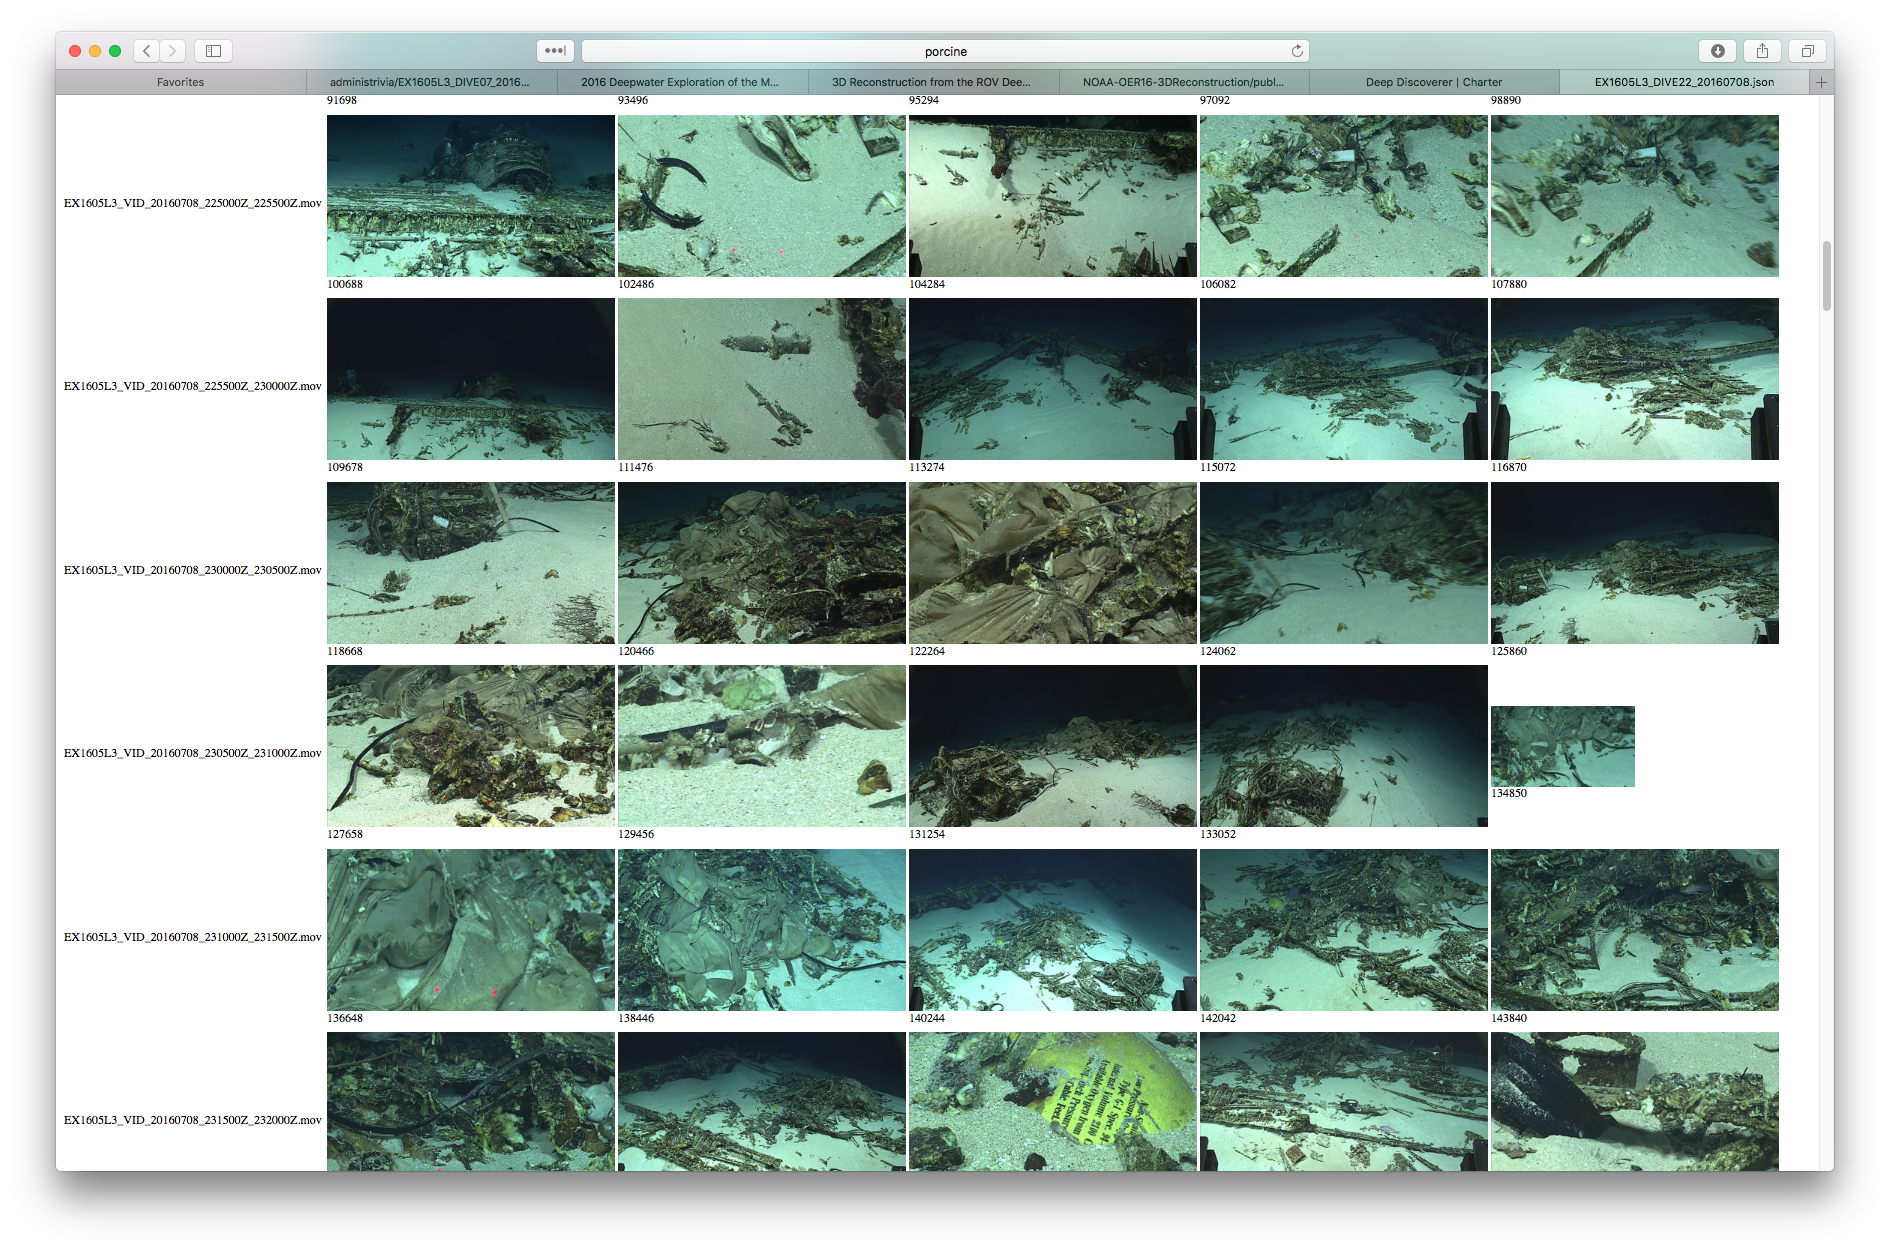
\includegraphics[width=\textwidth]{images/thumbnailer_screenshot.png}
    \caption{Screenshot from video synopsis for dive EX1605L3\_DIVE22.   Constituent video files are shown in leftmost column.   One thumbnail image is drawn for every minute of video.  The number under each thumbnail give that frame's sequence within the dive, indexed from the beginning of the first video in the dive.}
    \label{img:thumbnails}
\end{figure}

This strategy was selected to allow for documented, repeatable delineation and extraction of subsets from a given video.  Using this tool, a small number of test subsets were identified, with initial work quickly narrowed to just two dives: EX1605L3\_DIVE4 and EX1605L3\_DIVE22.  For each dive, an additional meta-data records was generated in JSON format.  The ``synopsis'' format:

\begin{Verbatim}[fontsize=\small]
{
  "source": "$NOAA_DIR/EX1605L3/EX1605L3_DIVE22_20160708/Full/EX1605L3_DIVE22_20160708.json",
  "chunks": {
    "descending": {
      "range": {  "start": 1  }
    },
    "approaching bottom": {
      "range": { "start": 38800 }
    },
    "approaching wing": {
      "range": { "start": 58800 }
    },
    "engine one": {
      "range": { "start": 63500 }
    },
    "landing gear": {
      "range": { "start": 71500 }
    },
    ...
\end{Verbatim}


\noindent allows definition of predefined ``regions'' or ``bookmarks'' within a video, for later access, with both EX1605L3\_DIVE4 and EX1605L3\_DIVE22 annotated in this manner.  A second file format allows designation of specific frame numbers to be extracted from a dive and automatically added to a Photoscan project.

\subsubsection{Post-Processed Reconstruction}

A segment from each video was selected for reconstruction using Agisoft Photoscan.   Within dive EX1605L3\_DIVE4, three consecutive periods of interest, labelled as ``hillside'', ``upslope'' and ``top of slope'' were examined.   ``Hillside'' starts with the ROV advancing towards a rocky slope (figure \ref{fig:ex1605l3_dive4_hillside_begin}), then transiting laterally to the right along the slope face.  At the conclusion of ``hillside'', the main science camera zooms in and examines a geologic feature while the ROV continues to move upslope, which is designated ``upslope''.  It then zooms back out and the ROV continues to explore further upslope.  At the conclusion of this section, the ROV ascends away from the topography into open water and the seafloor is no longer visible (figure \ref{fig:ex1605l3_dive4_top_of_slope_end}).  Images sets sere extracted from each segment at a rate of approximately one image per 100 frames (approx. 3 seconds).

\begin{figure}[p]
    \centering
    \begin{subfigure}[b]{0.48\textwidth}
        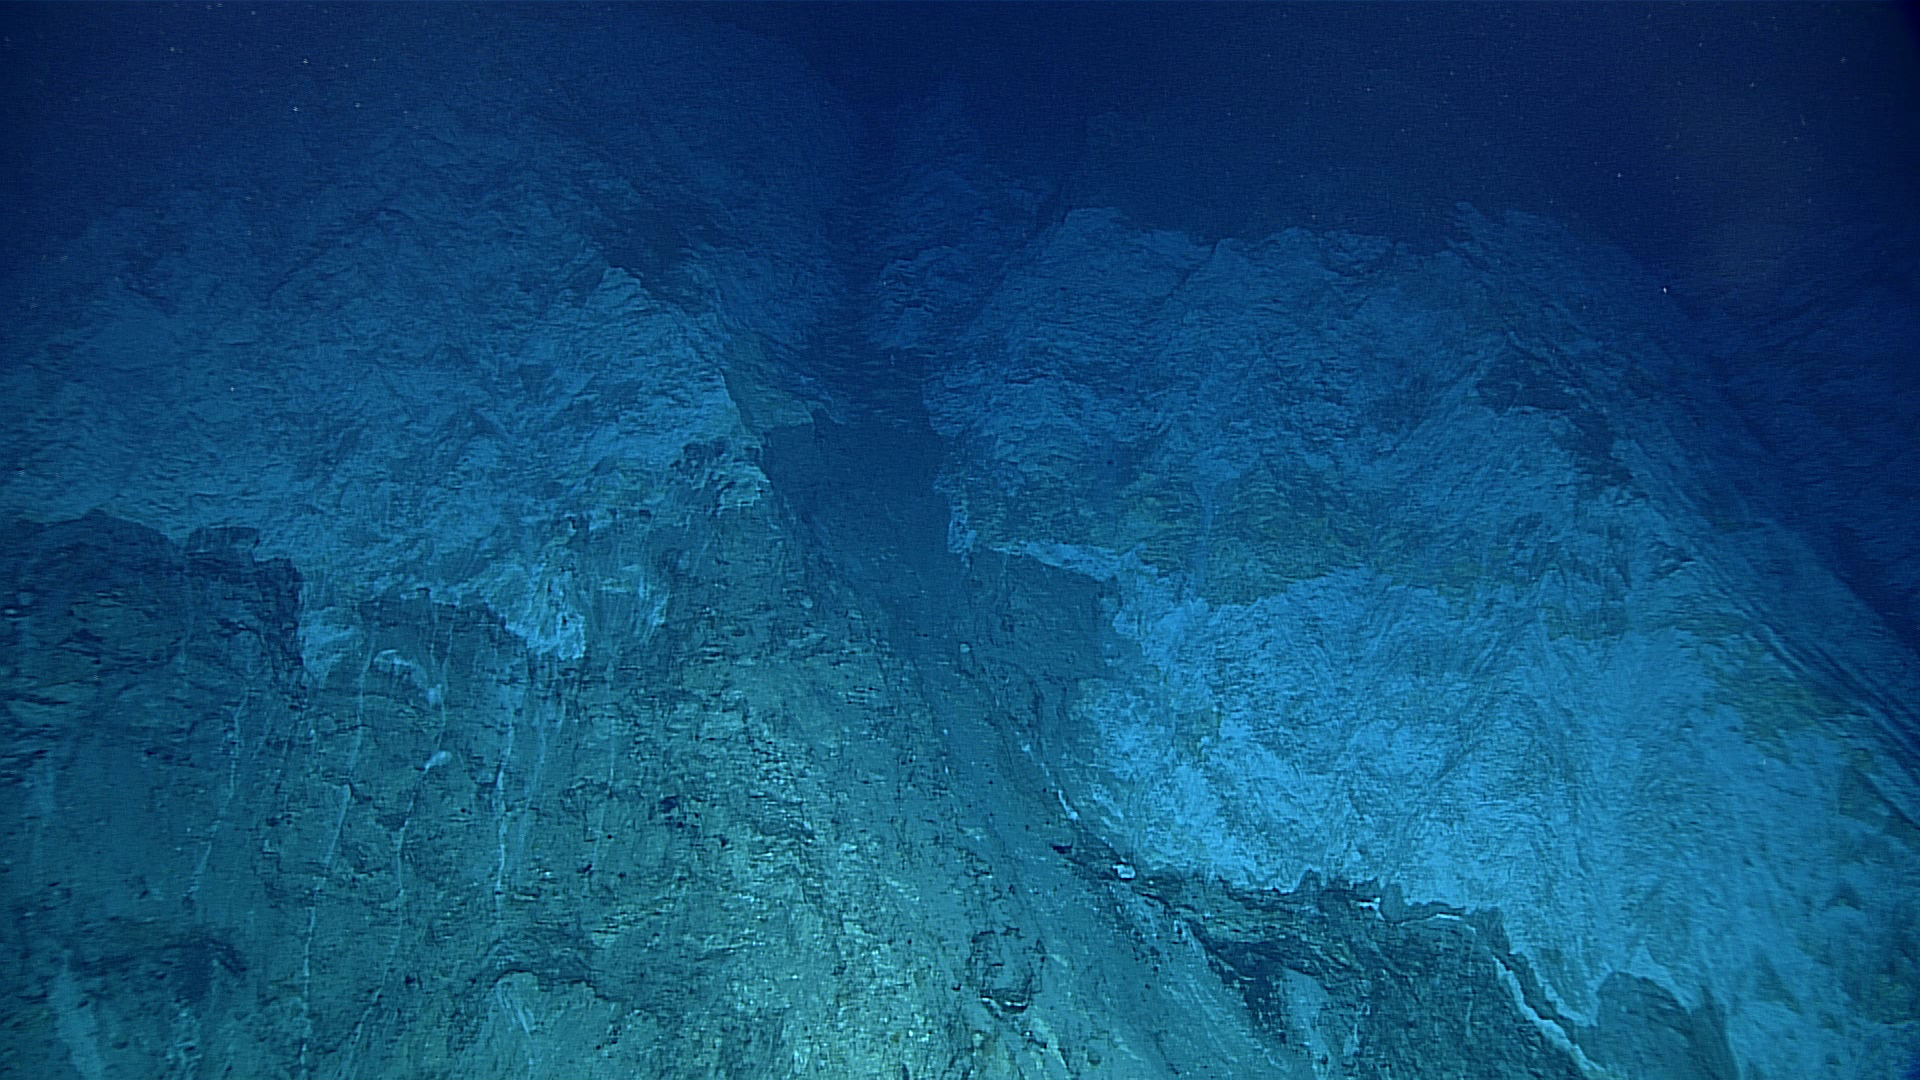
\includegraphics[width=\textwidth]{images/image_643000.png}
        \caption{Frame 643000.}
        \label{fig:ex1605l3_dive4_hillside_begin}
    \end{subfigure}
    \begin{subfigure}[b]{0.48\textwidth}
        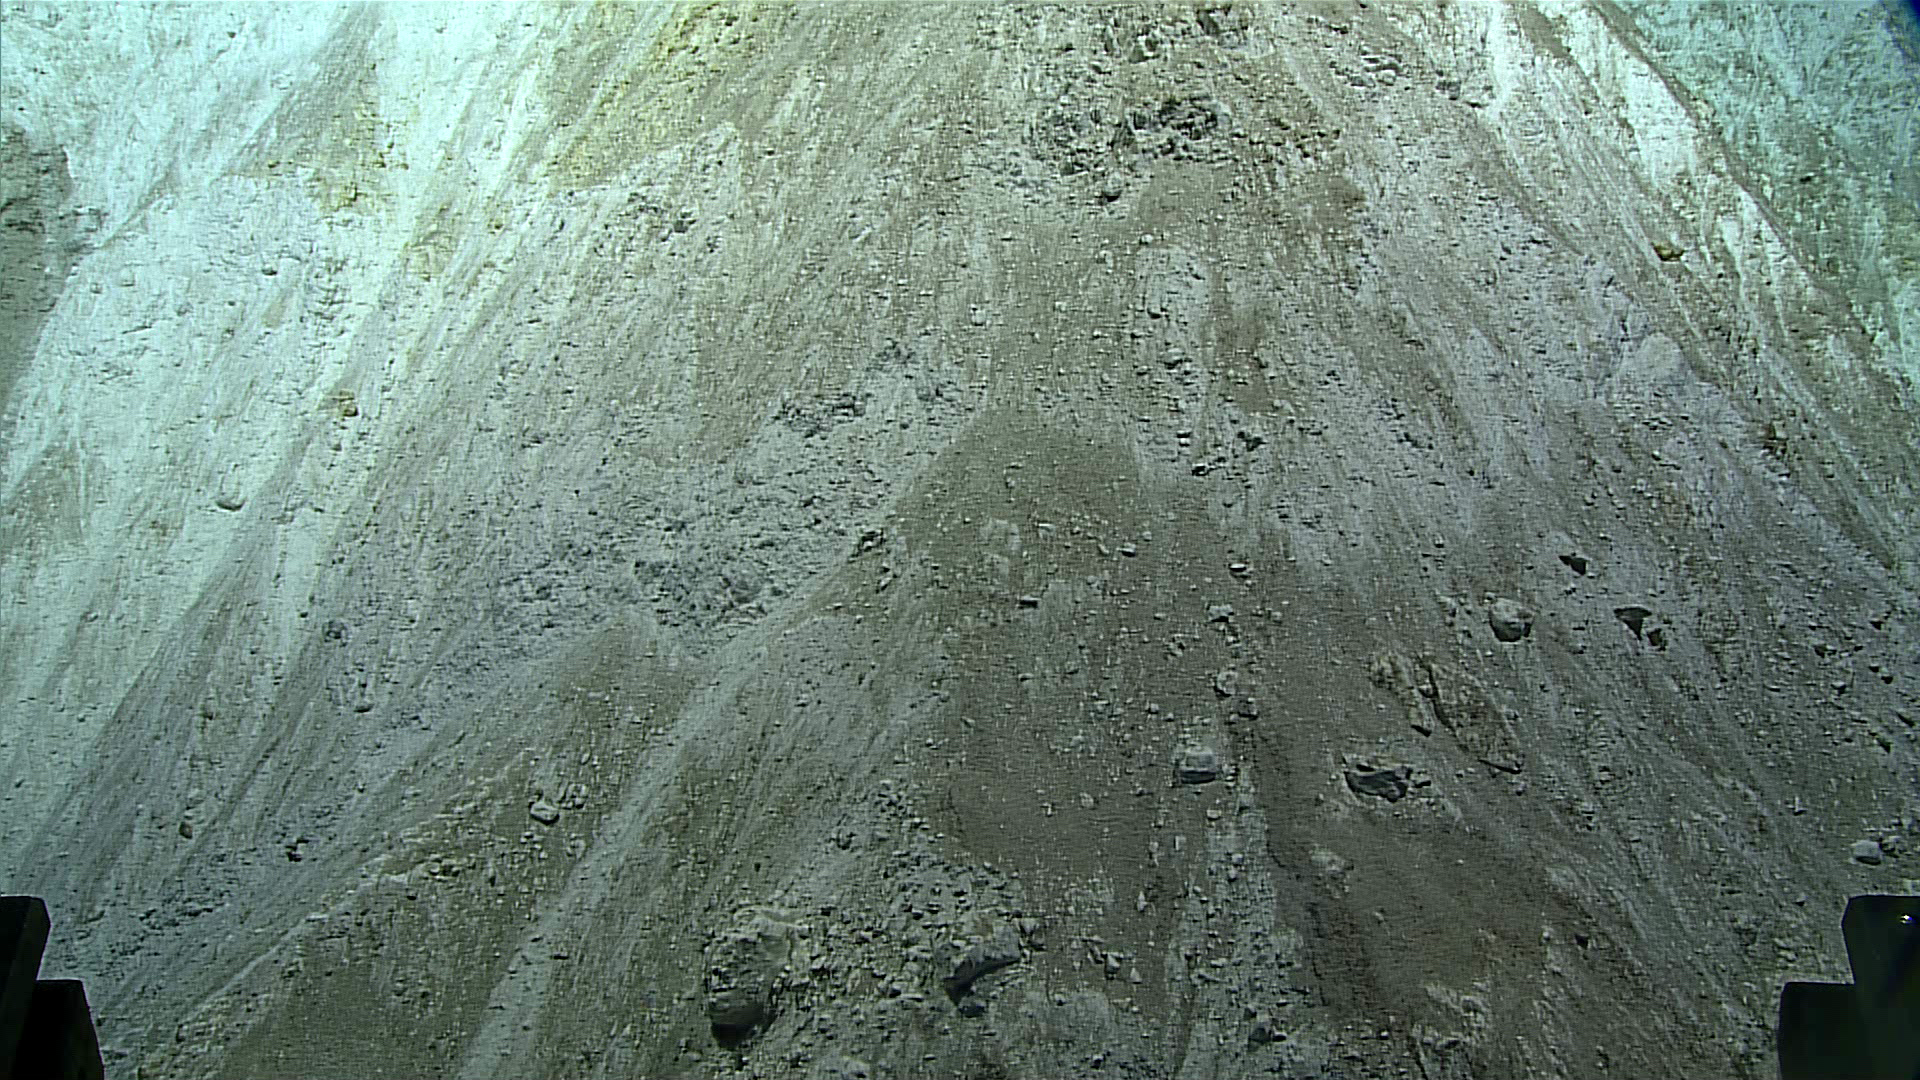
\includegraphics[width=\textwidth]{images/image_651100.png}
        \caption{Frame 651100.}
        \label{fig:ex1605l3_dive4_hillside_end}
    \end{subfigure}
    \caption{First and last images in ``hillside'' segment within dive EX1605L3\_DIVE4.}
\end{figure}

\begin{figure}[p]
    \centering
    \begin{subfigure}[b]{0.48\textwidth}
        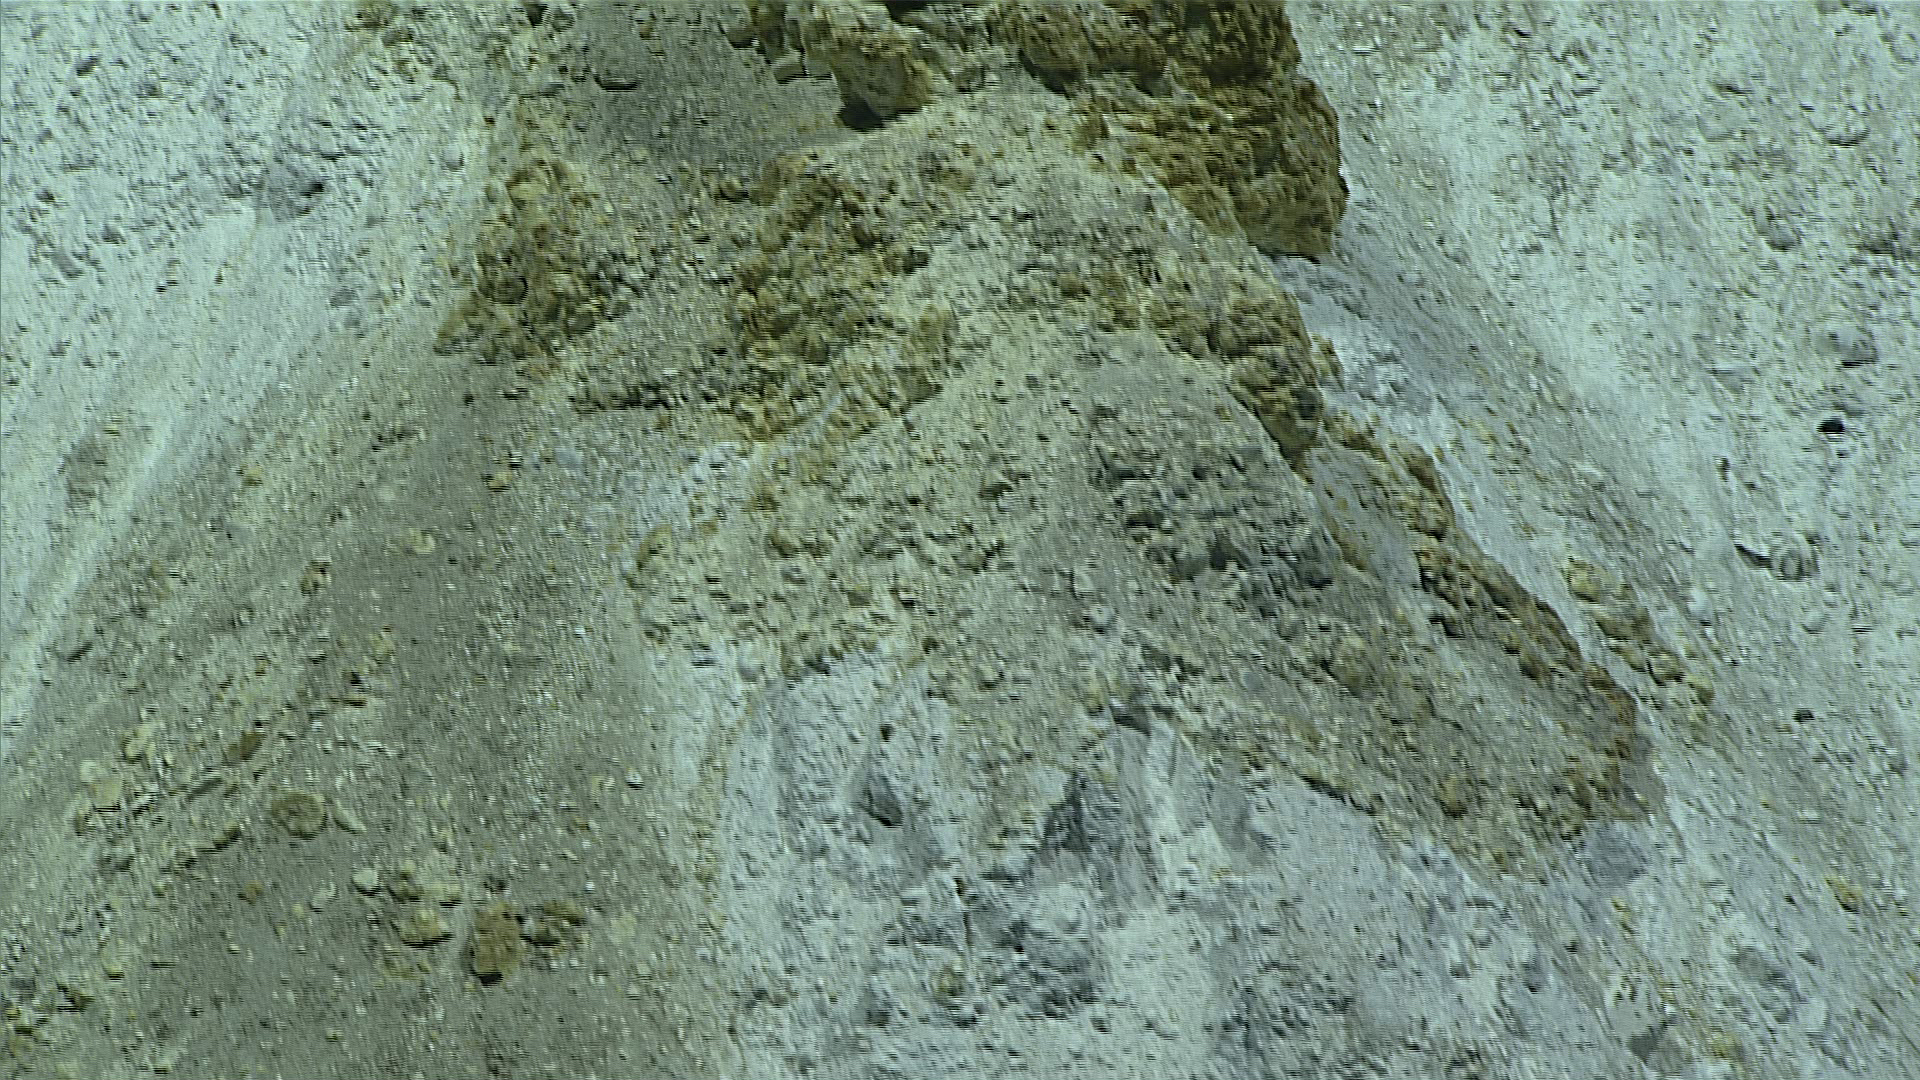
\includegraphics[width=\textwidth]{images/image_653000.png}
        \caption{Frame 653000.}
        \label{fig:ex1605l3_dive4_upslope_begin}
    \end{subfigure}
    \begin{subfigure}[b]{0.48\textwidth}
        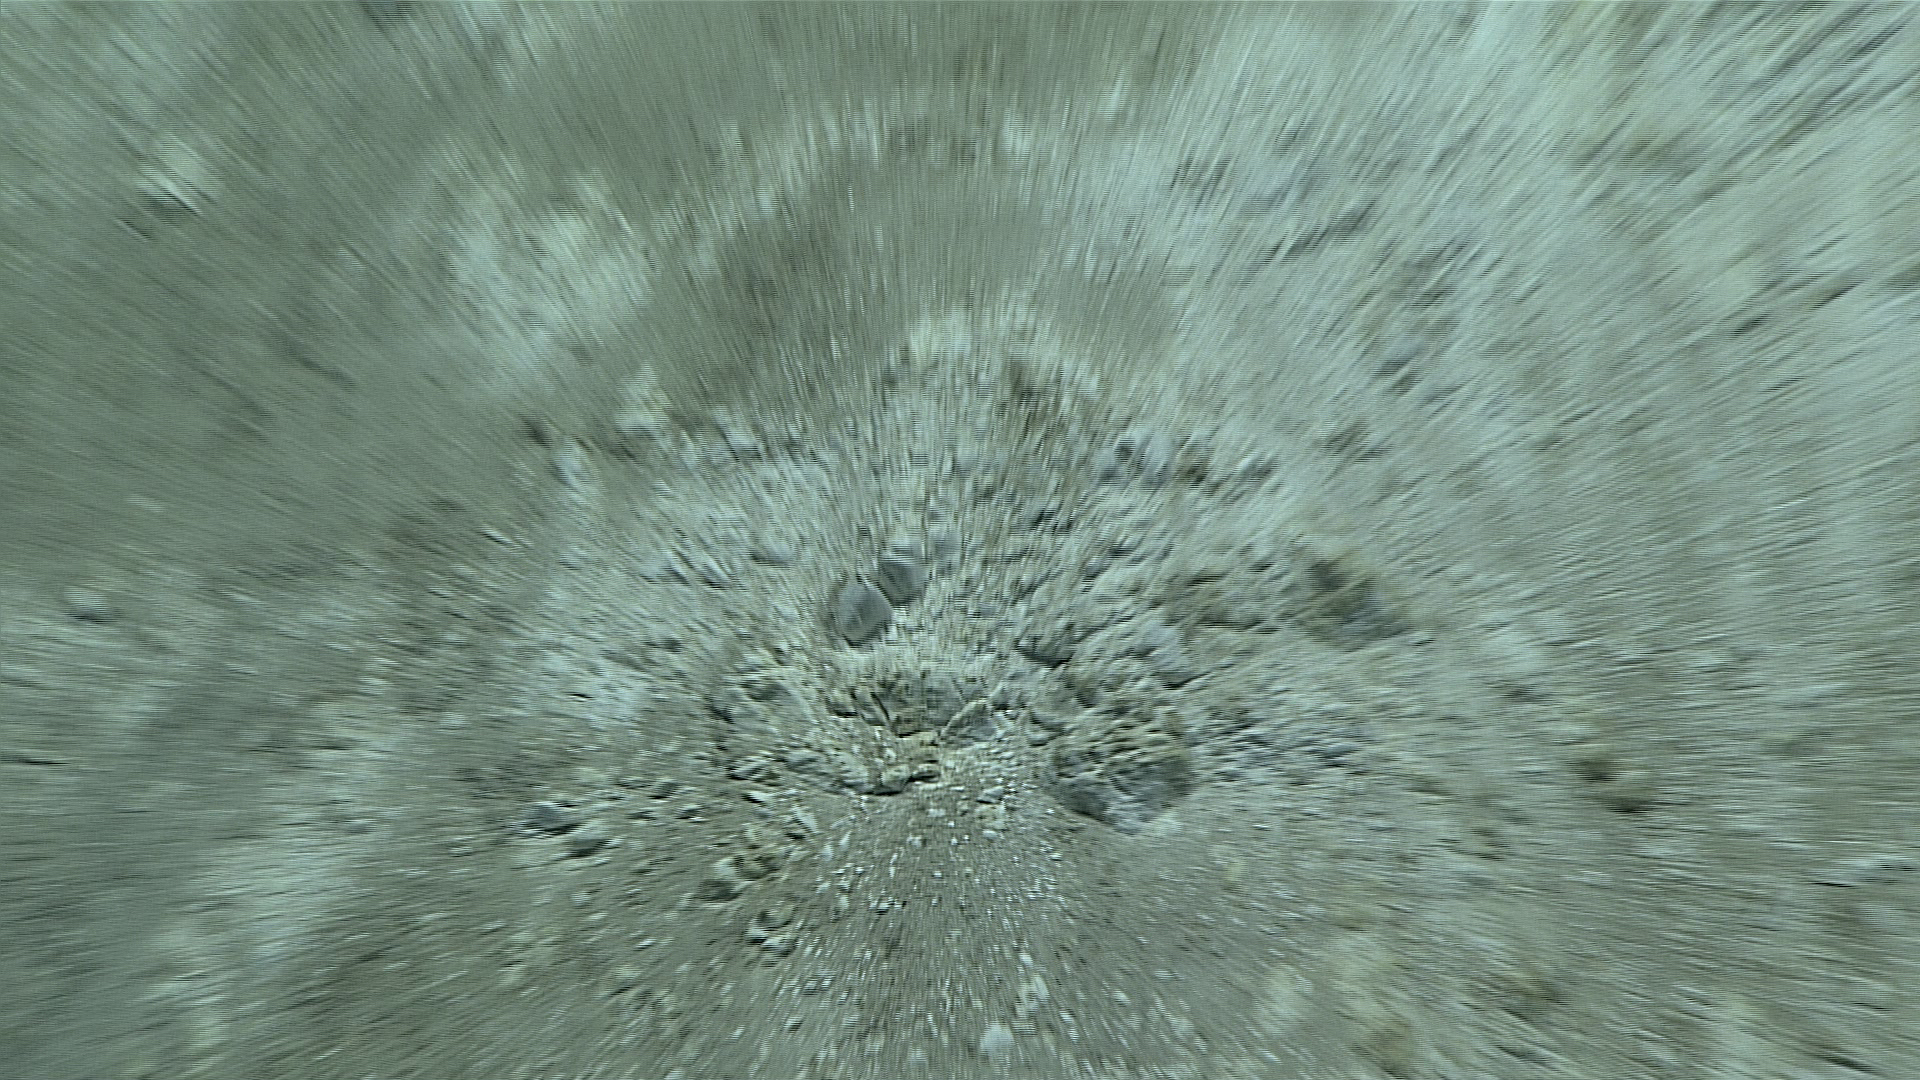
\includegraphics[width=\textwidth]{images/image_656500.png}
        \caption{Frame 656500.}
        \label{fig:ex1605l3_dive4_upslope_end}
    \end{subfigure}
    \caption{First and last images in ``upslope'' segment within dive EX1605L3\_DIVE4.}
\end{figure}

\begin{figure}[p]
    \centering
    \begin{subfigure}[b]{0.48\textwidth}
        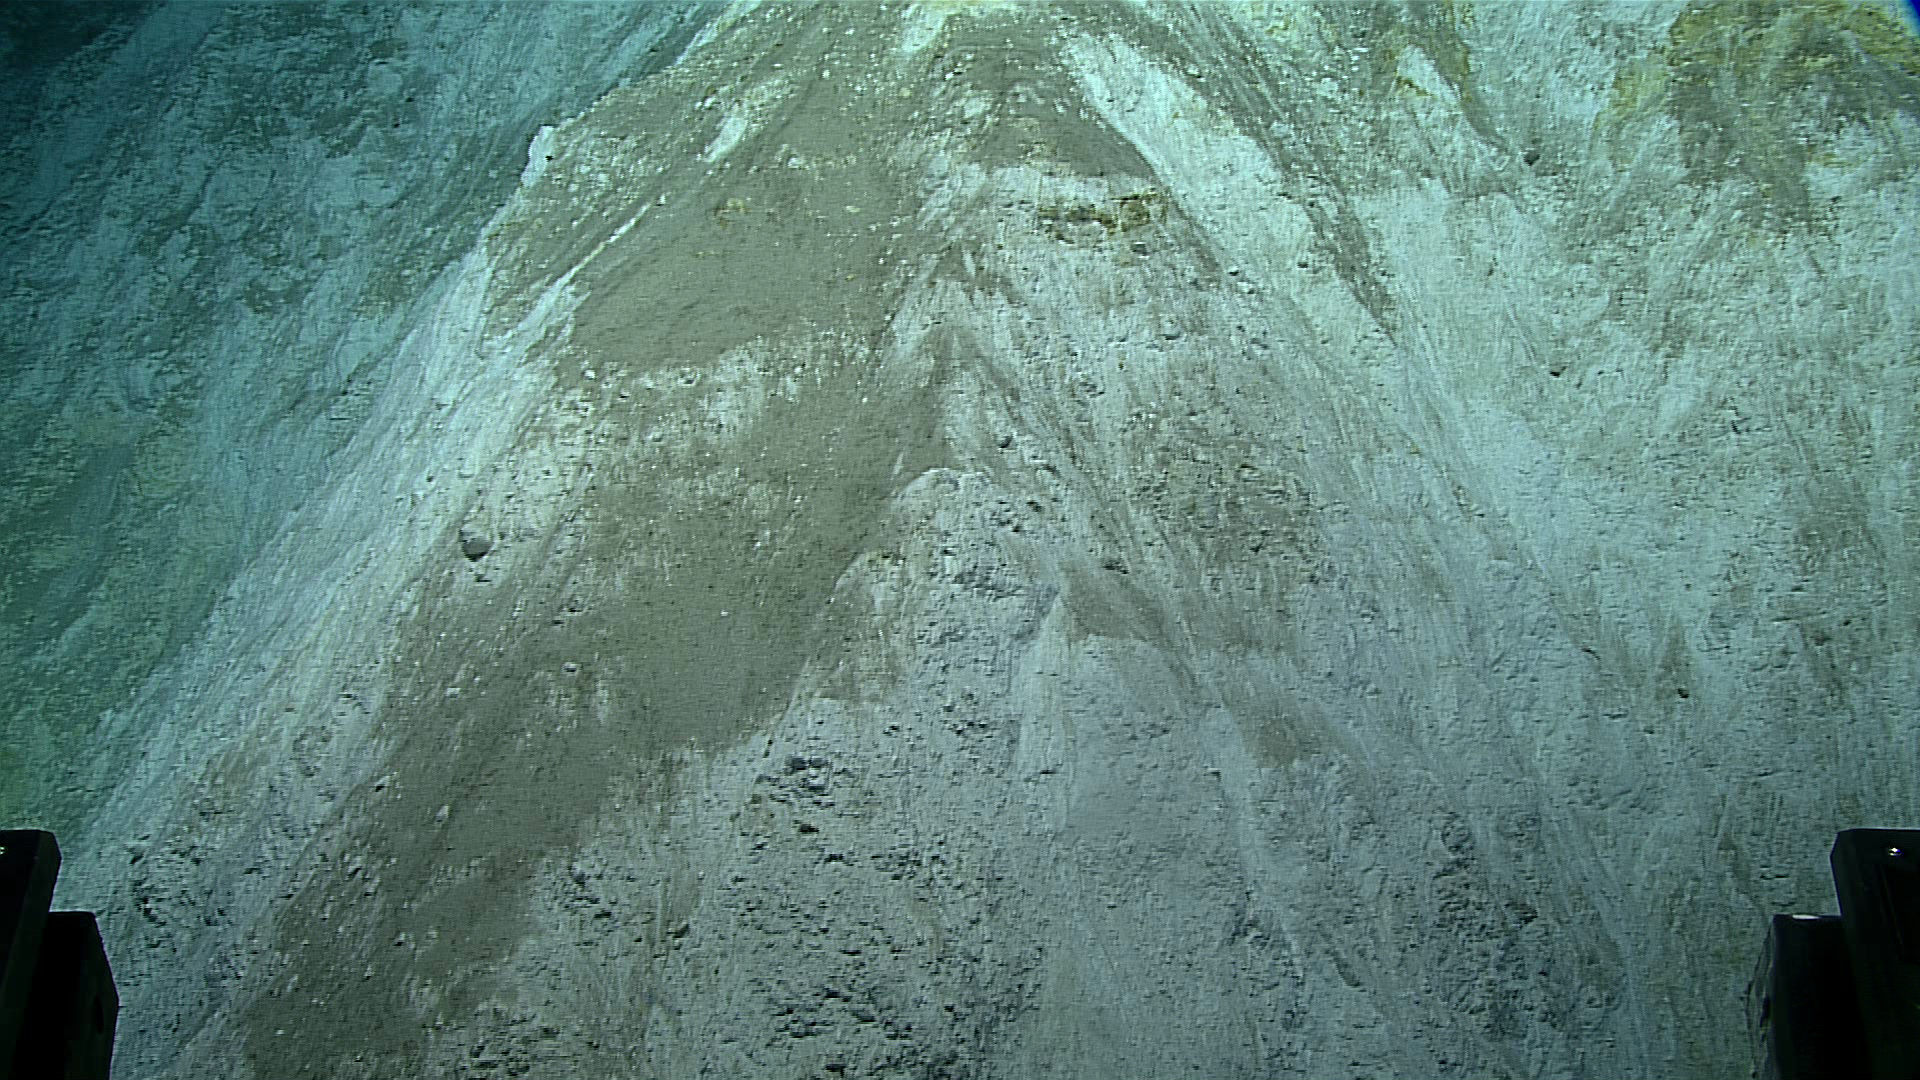
\includegraphics[width=\textwidth]{images/image_656700.png}
        \caption{Frame 656700.}
        \label{fig:ex1605l3_dive4_top_of_slope_begin}
    \end{subfigure}
    \begin{subfigure}[b]{0.48\textwidth}
        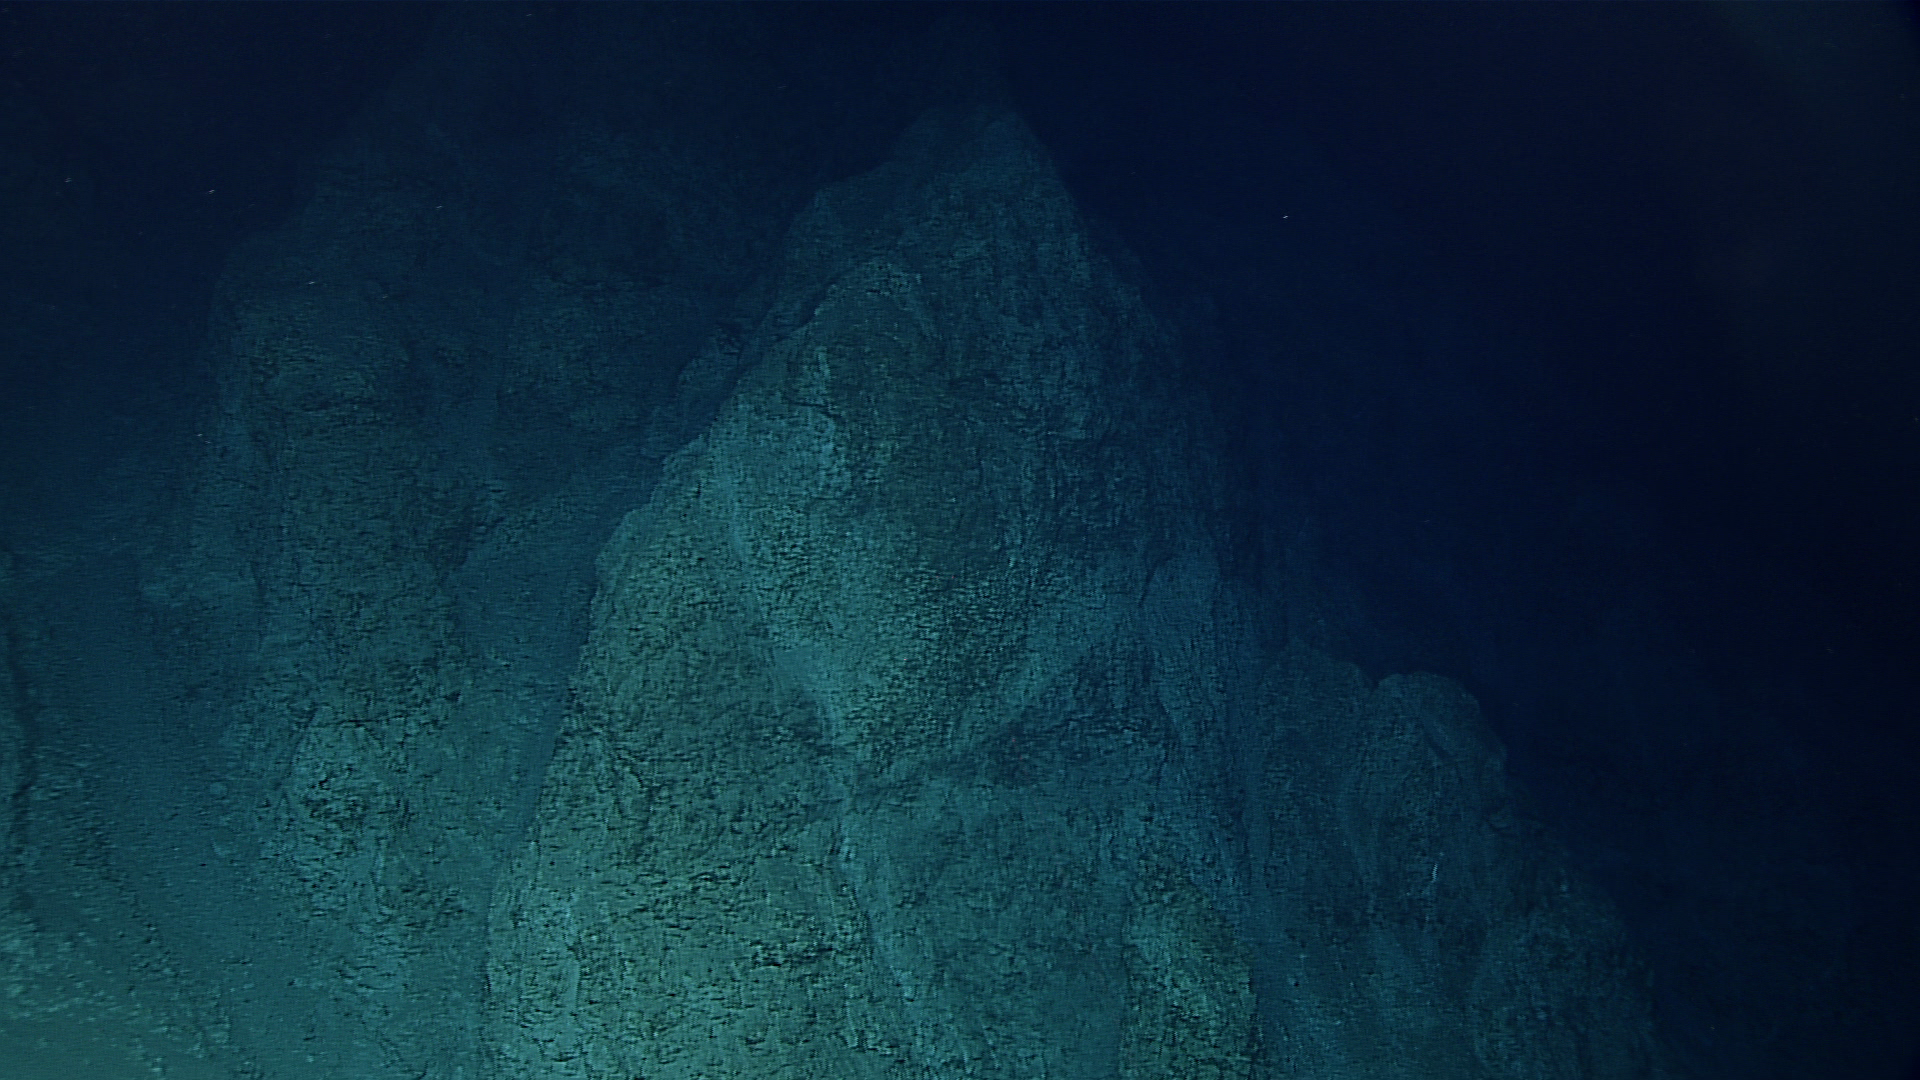
\includegraphics[width=\textwidth]{images/image_679900.png}
        \caption{Frame 679900.}
        \label{fig:ex1605l3_dive4_top_of_slope_end}
    \end{subfigure}
    \caption{First and last image in ``top of slope'' segment within dive EX1605L3\_DIVE4.}
\end{figure}

A total of 82 images were extracted from ``hillside.'' and were successfully reconstructed in Photoscan as shown in Figures \ref{fig:hillside_photoscan} and \ref{fig:hillside_photoscan_trajectory}.  Figure \ref{fig:hillside_photoscan_trajectory} shows the estimated trajectory of the camera (ROV) as derived from the imagery.  This estimated trajectory is qualitatively correct, showing the ROV approaching the hillside (as bottom of image), then transiting rightward across a gully to another ridge.   

\begin{figure}
    \centering
    \begin{subfigure}[b]{0.95\textwidth}
        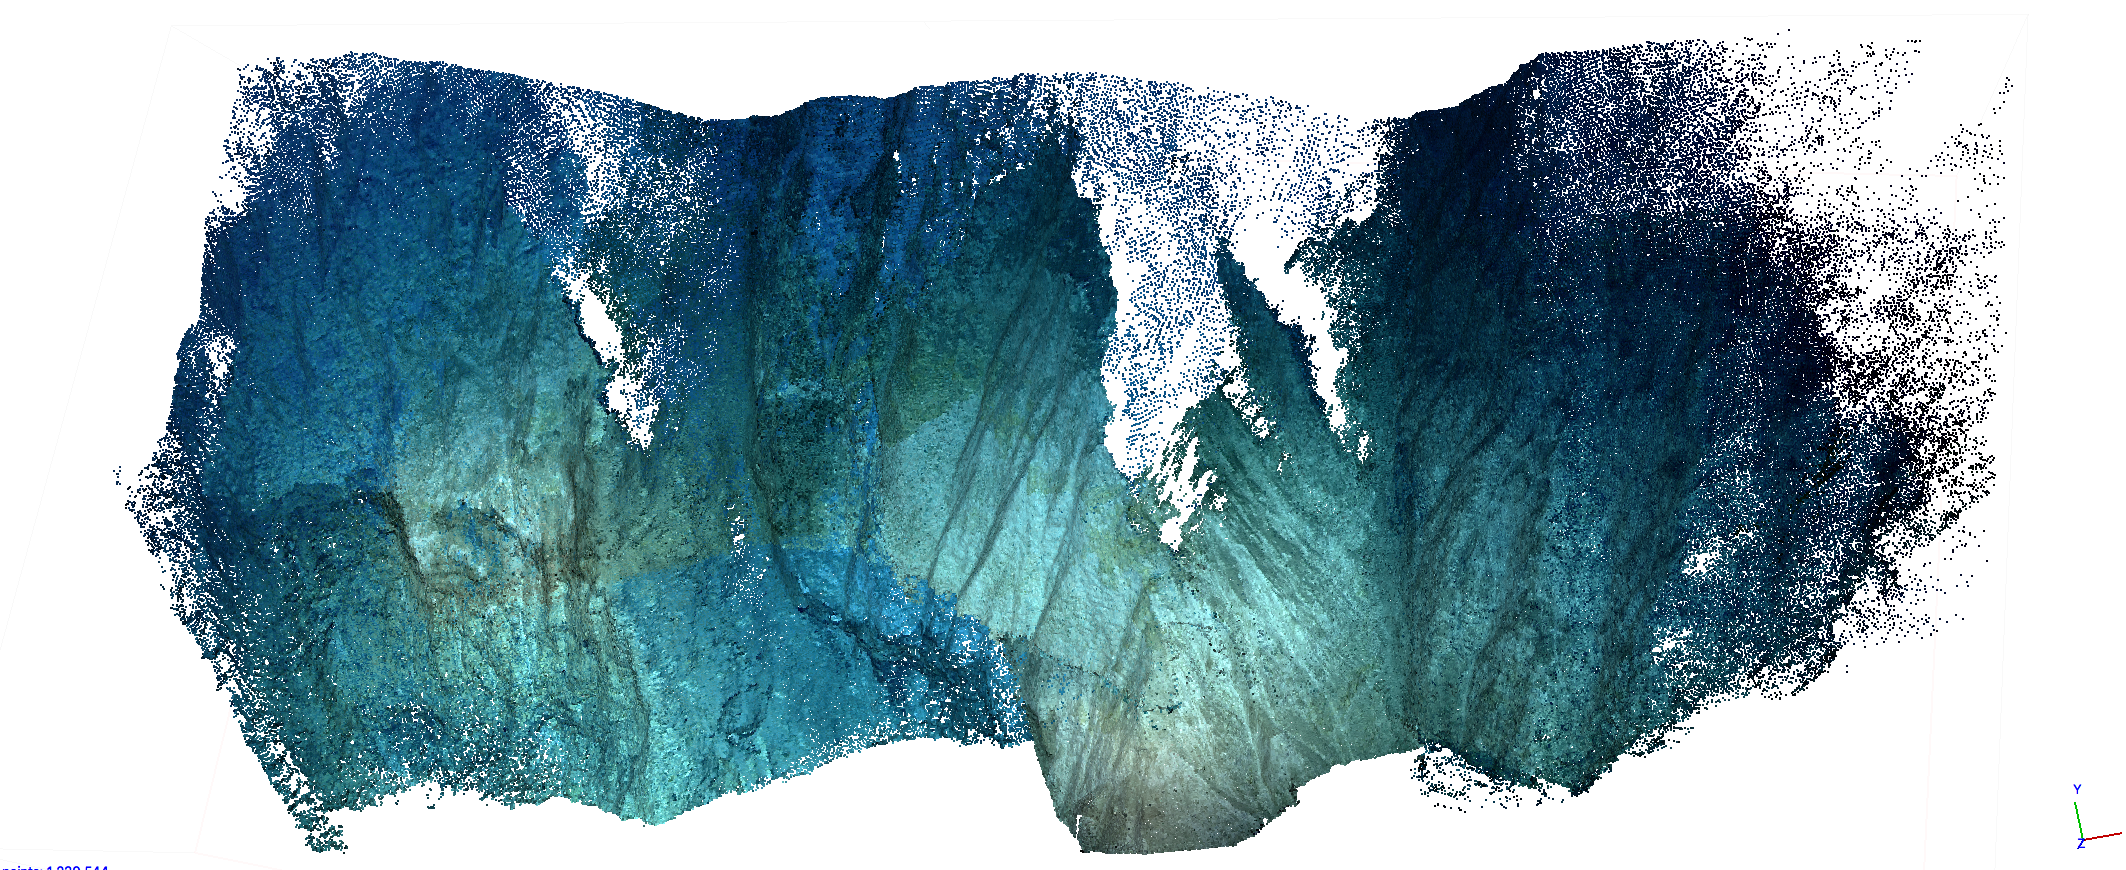
\includegraphics[width=\textwidth]{images/hillside_reconstruction.png}
        \caption{Dense point cloud from reconstruction of ``hillside'' segment.}
        \label{fig:hillside_photoscan}
    \end{subfigure}
    \\[24pt]
    \begin{subfigure}[b]{0.95\textwidth}
        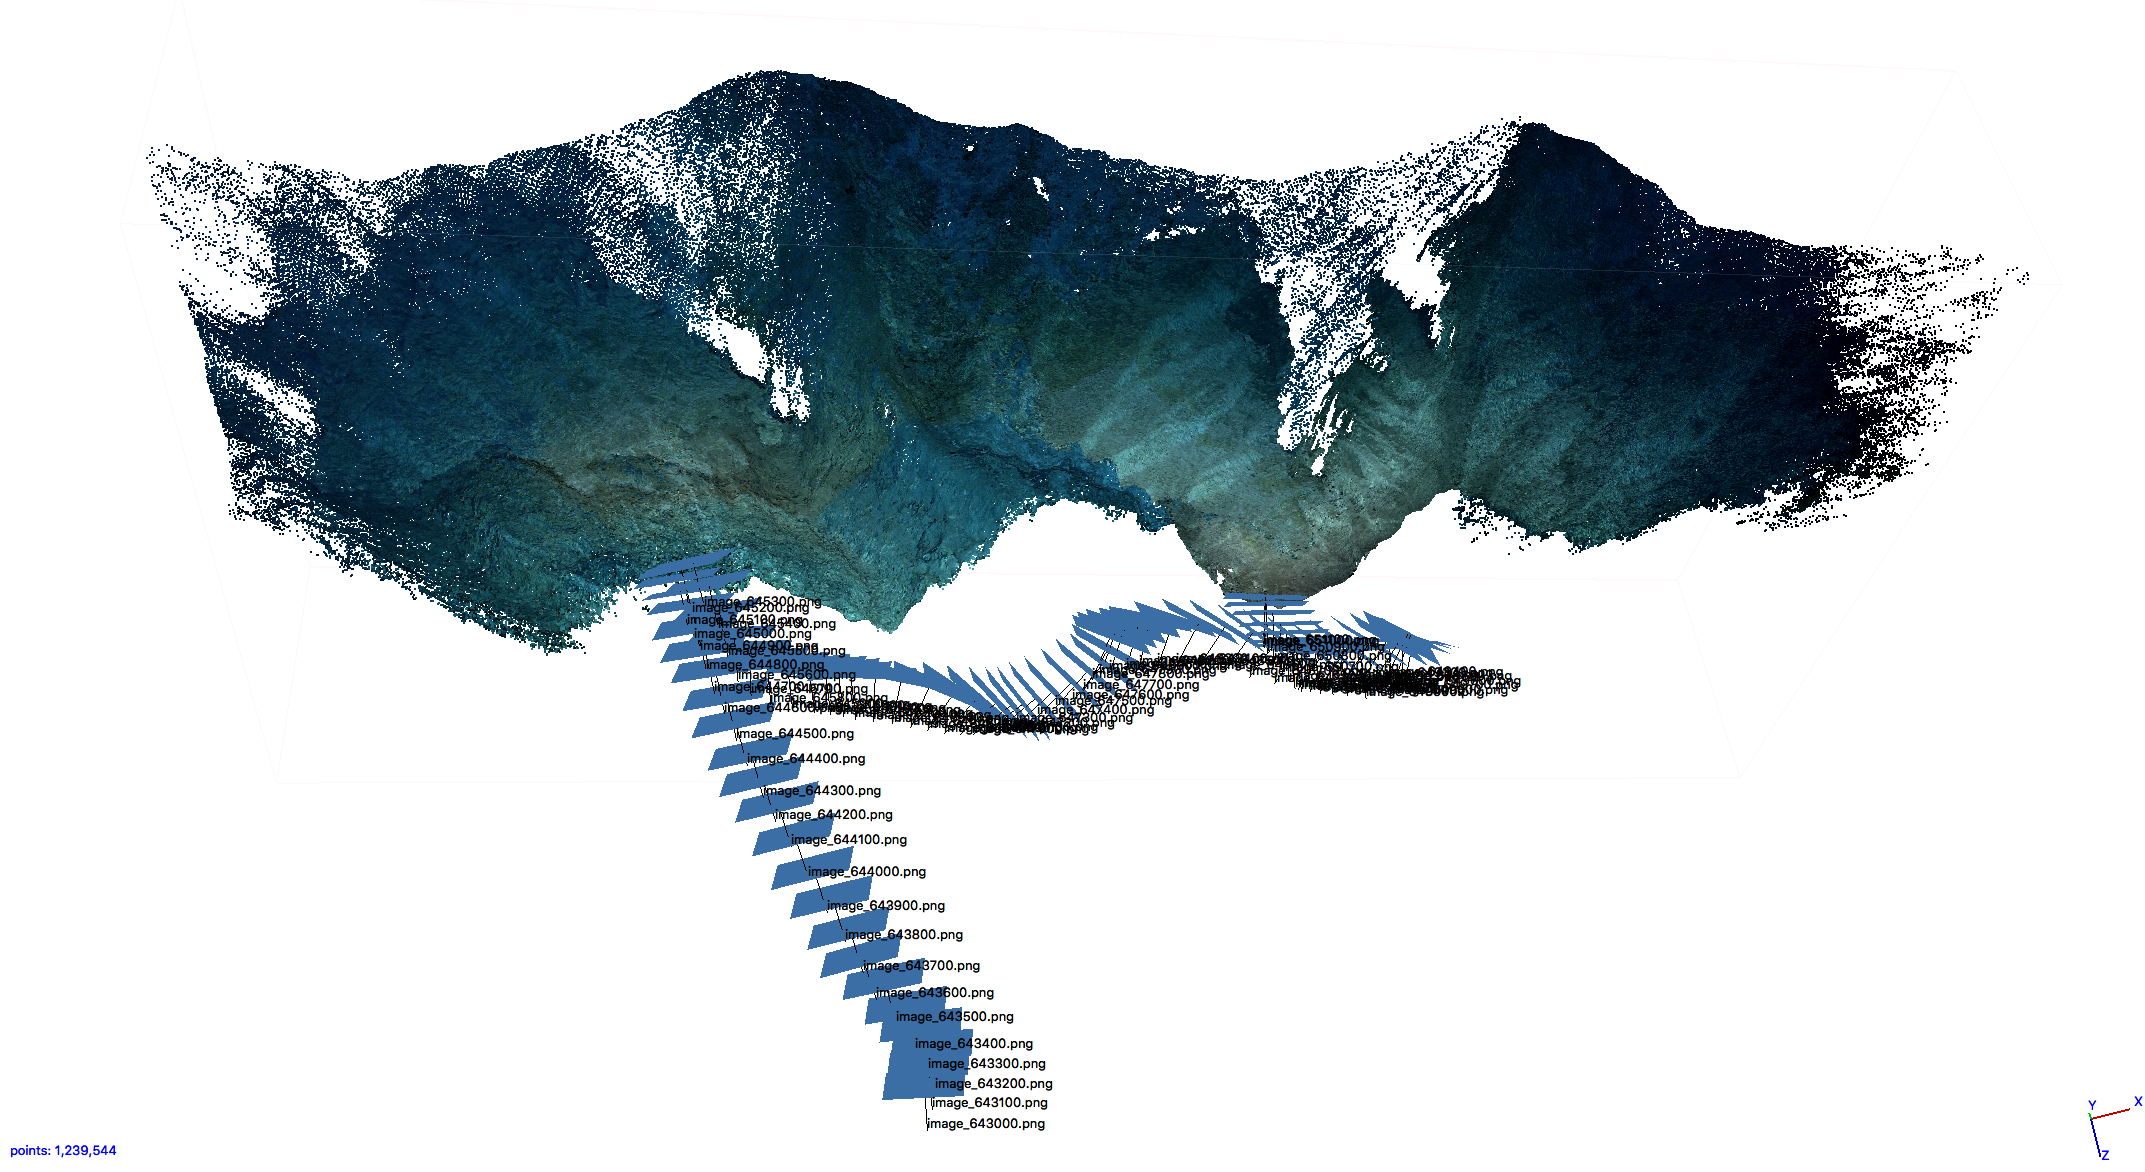
\includegraphics[width=\textwidth]{images/hillside_reconstruction_trajectory.png}
        \caption{Dense point cloud of ``hillside'' with estimated position of camera for each input image (shown as purple squares) overlaid.  Relative to figure \ref{fig:hillside_photoscan}, the top edge of model has been pitched towards the observer.  This view shows the estimated camera motion, approaching the hillside (to left), then transiting left-to-right across the slope face.}
        \label{fig:hillside_photoscan_trajectory}
    \end{subfigure}
    \caption{Reconstructions for ``hillside'' segment within dive EX1605L3\_DIVE4.}
\end{figure}

While qualitatively successful, this reconstruction illustrates many of the issues observed while reconstructing the ROV video.    Water clarity at depth (approx. 6000m in this case) is very good, with little turbidity, however, the strong absorption of light creates an unmodelled distortion which is unique to underwater imagery.   In standard terrestrial imagery, the scene is generally evenly lit, often by natural light and there is generally no dependency between the ``quality'' of the imagery of a given object and its distance from the camera, and instead the limits of reconstruction are a function solely of camera resolution.   In the ROV video, where the only light is provided by the ROV itself, distant objects undergo a fading in color and contrast well before they become too small to resolve.   For example, in ``hillside,'' the seafloor is initially far from the ROV and is primarily blue-black in color (as in figure \ref{fig:ex1605l3_dive4_hillside_begin}).  As the ROV approaches, the optical path through the water decreases in length and the apparent color of the slope becomes the ``true'' brown-grey.   Despite this shifting appearance, Photoscan is able to form image correspondences (in part because the underlying image matching algorithms work in greyscale), however, the impact of this color shifting can be seen in the mottled appearance of Figure \ref{fig:hillside_photoscan}. 
Portions of the scene which are only seen from a distance (e.g., the upper and lower left, and far right of the model) are rendered in blue, while portions seen at close-range at some point during the transit appear closer to their true color.   Portions of the slope only viewed at the edges of the light, for example, the far right, become increasingly indistinct.  Similarly, the right faces of the two ridges are undefined because the ROV is generally yawed rightwards relative to the normal to the slope face and does not view these portions of the topography.     Such an omission might have been avoided given real-time reconstruction, where such a data gap would be immediately noticed.

A similar reconstruction from the 130 images extracted from ``top of slope'' is shown in figure \ref{fig:top_of_slope_photoscan}.  As with ``hillside,'' the reconstruction is successful, capturing details of the topography as the ROV cross between ridges.   As shown in figure \ref{fig:top_of_slope_photoscan_trajectory}, the ROV starts at the lower right of the model, then ascends upwards and to the left, before moving upwards and away from the seafloor while over the ridge at model center.  As with the ``hillside'' reconstructions, this model is subject to the same color banding based on the closest approach of the ROV to the feature.

\begin{figure}
    \centering
    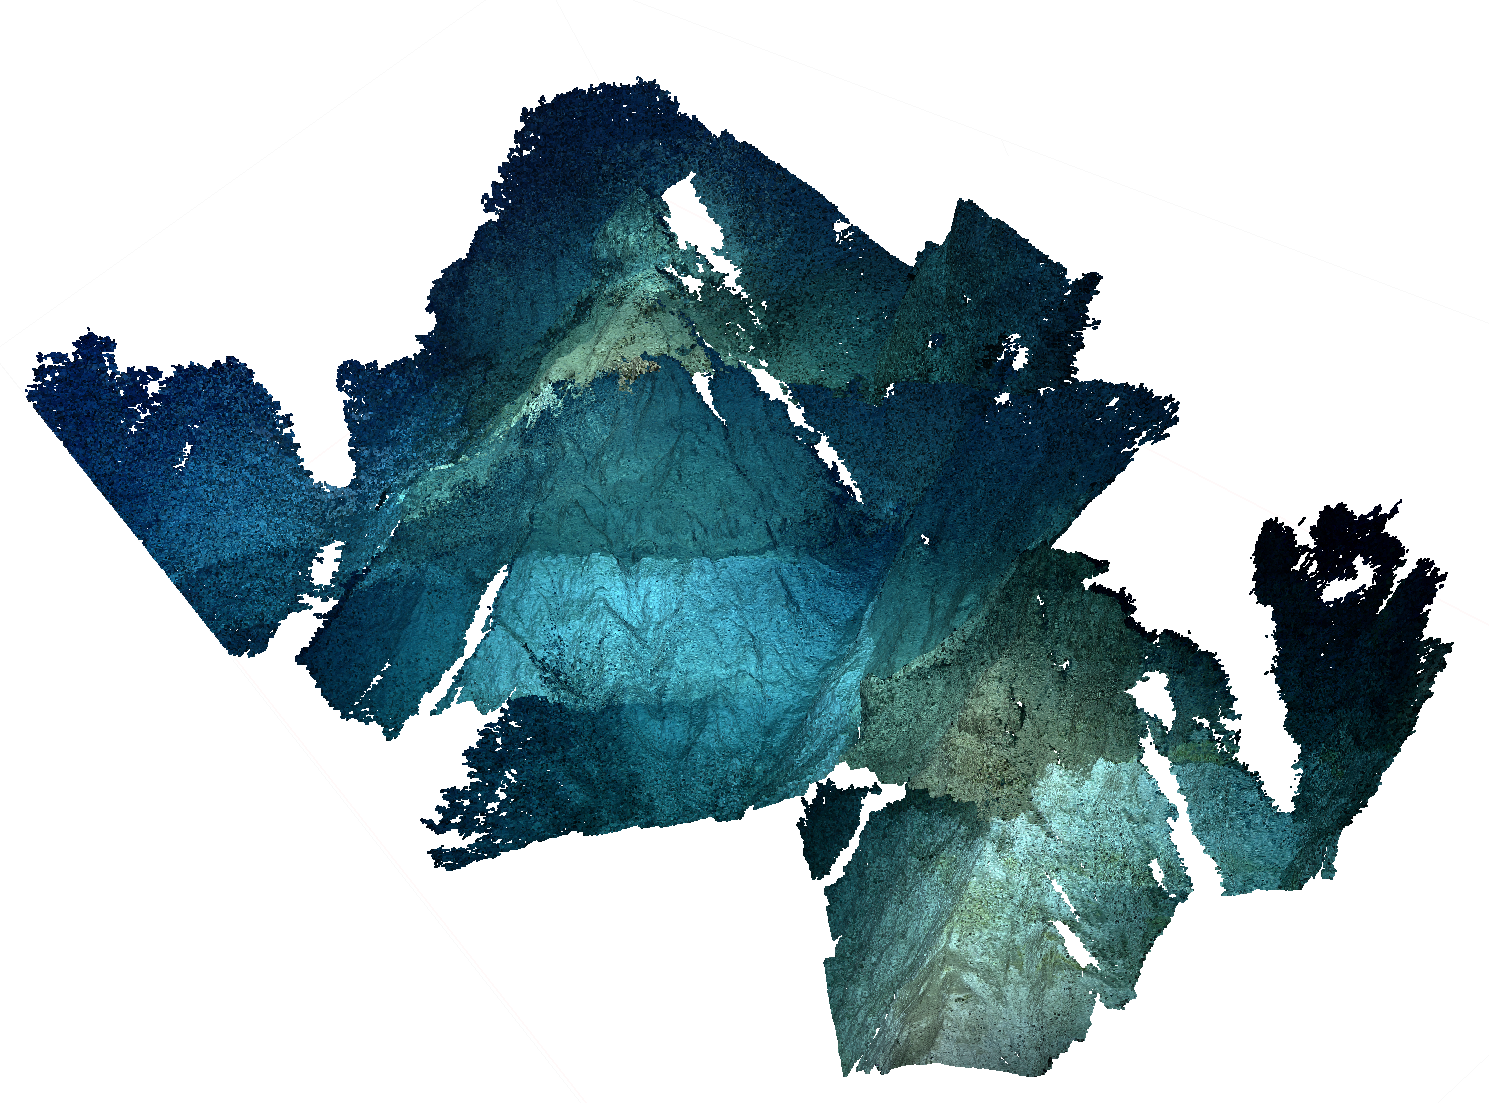
\includegraphics[width=0.95\textwidth]{images/top_of_slope_reconstruction.png}
    \caption{Reconstruction of ``top\_of\_slope'' segment within EX1605L3\_DIVE4.}
    \label{fig:top_of_slope_photoscan}
\end{figure}

\begin{figure}
    \centering
    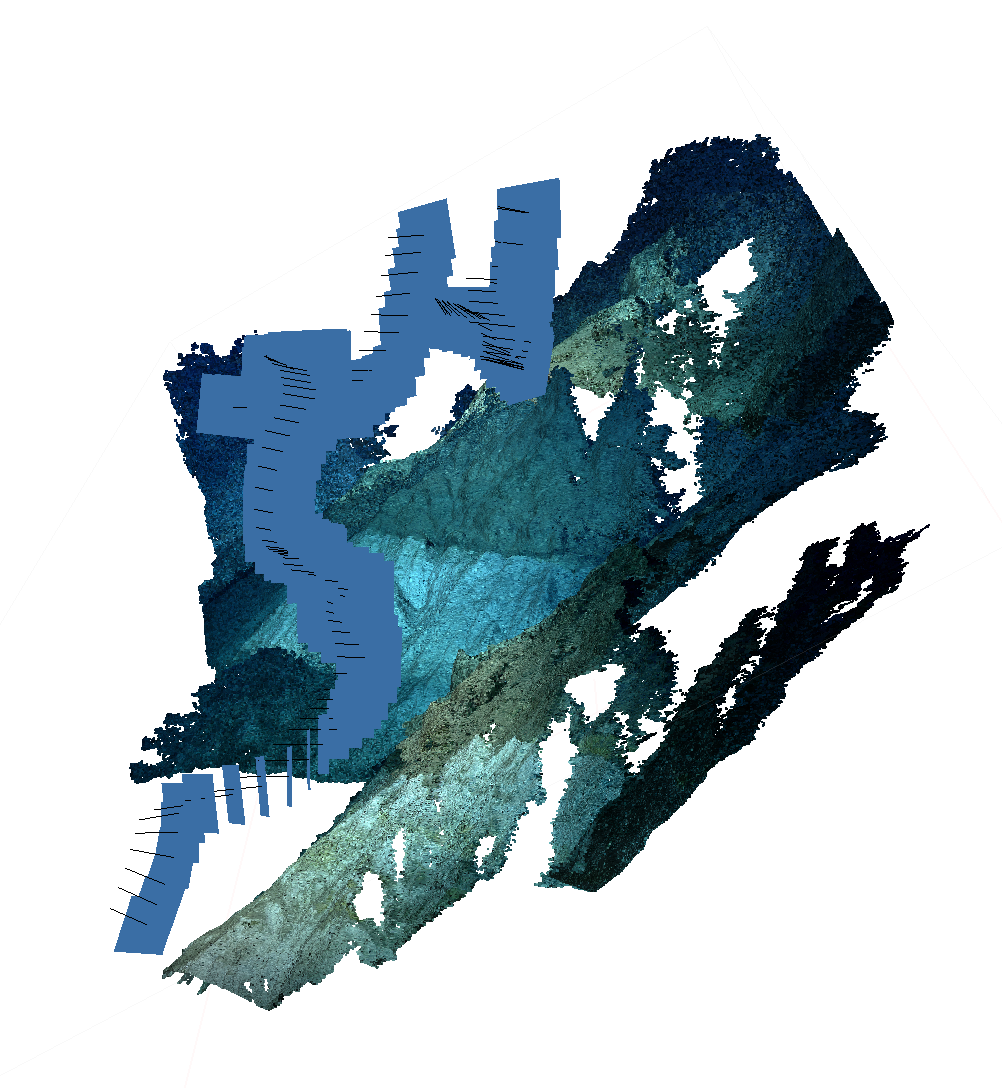
\includegraphics[width=0.95\textwidth]{images/top_of_slope_reconstruction_trajectory.png}
    \caption{Reconstruction of ``top\_of\_slope'' segment with overlaid camera trajectory.  Relative to figure \ref{fig:top_of_slope_photoscan}, the right side of the model has been pulled towards the observer.  The ROV starts at bottom of model and moves consistently upslope and away from the observer.}
    \label{fig:top_of_slope_photoscan_trajectory}
\end{figure}

While these two reconstructions are successful, several cautionary notes should be drawn from these models.   Most significantly, we have no way to verify the accuracy of the resulting topography and trajectories.    The larger message is the negative impact of the relatively short period of zoom-in ``upslope'' which effectively separates the ``hillside'' and ``top of slope'' segments.  While this short period is only approx. 3 minutes in length, the ROV moves sufficiently while zoomed-in such that there is no image overlap between ``hillside'' and ``top of slope'' which can be used to join the two models.  While is might be possible to join the two models via the estimated ROV motion within ``upslope'' it would be unlikely to be accurate and would represent a weak geometric constraint between the two larger models.   Again, this emphasizes the importance of multiple, overlapping images of a scene of interest.  This is particularly critical in linear transect missions such as this where a particular scene is unlikely to be viewed again to fill in the data gap.    In post-processing, the gap between ``hillside'' and ``top of slope'' could have been joined had the two mission segments intersected at any point, even if the time-ordered image sequence was not necessarily continuous.

\clearpage

Three consecutive segments were extracted from Dive EX1605L3\_DIVE22. ``approaching wing'' covers a period where the ROV is approaching an inverted B-29 site from off the starboard wingtip.  It then proceeds along the leading edge of the wing to the number one engine, leading to the segment ``engine one.''  This segment ends when the camera zooms into the engine to more closely examine the wreckage in segment ``engine detail.''

\begin{figure}[p]
    \centering
    \begin{subfigure}[b]{0.48\textwidth}
        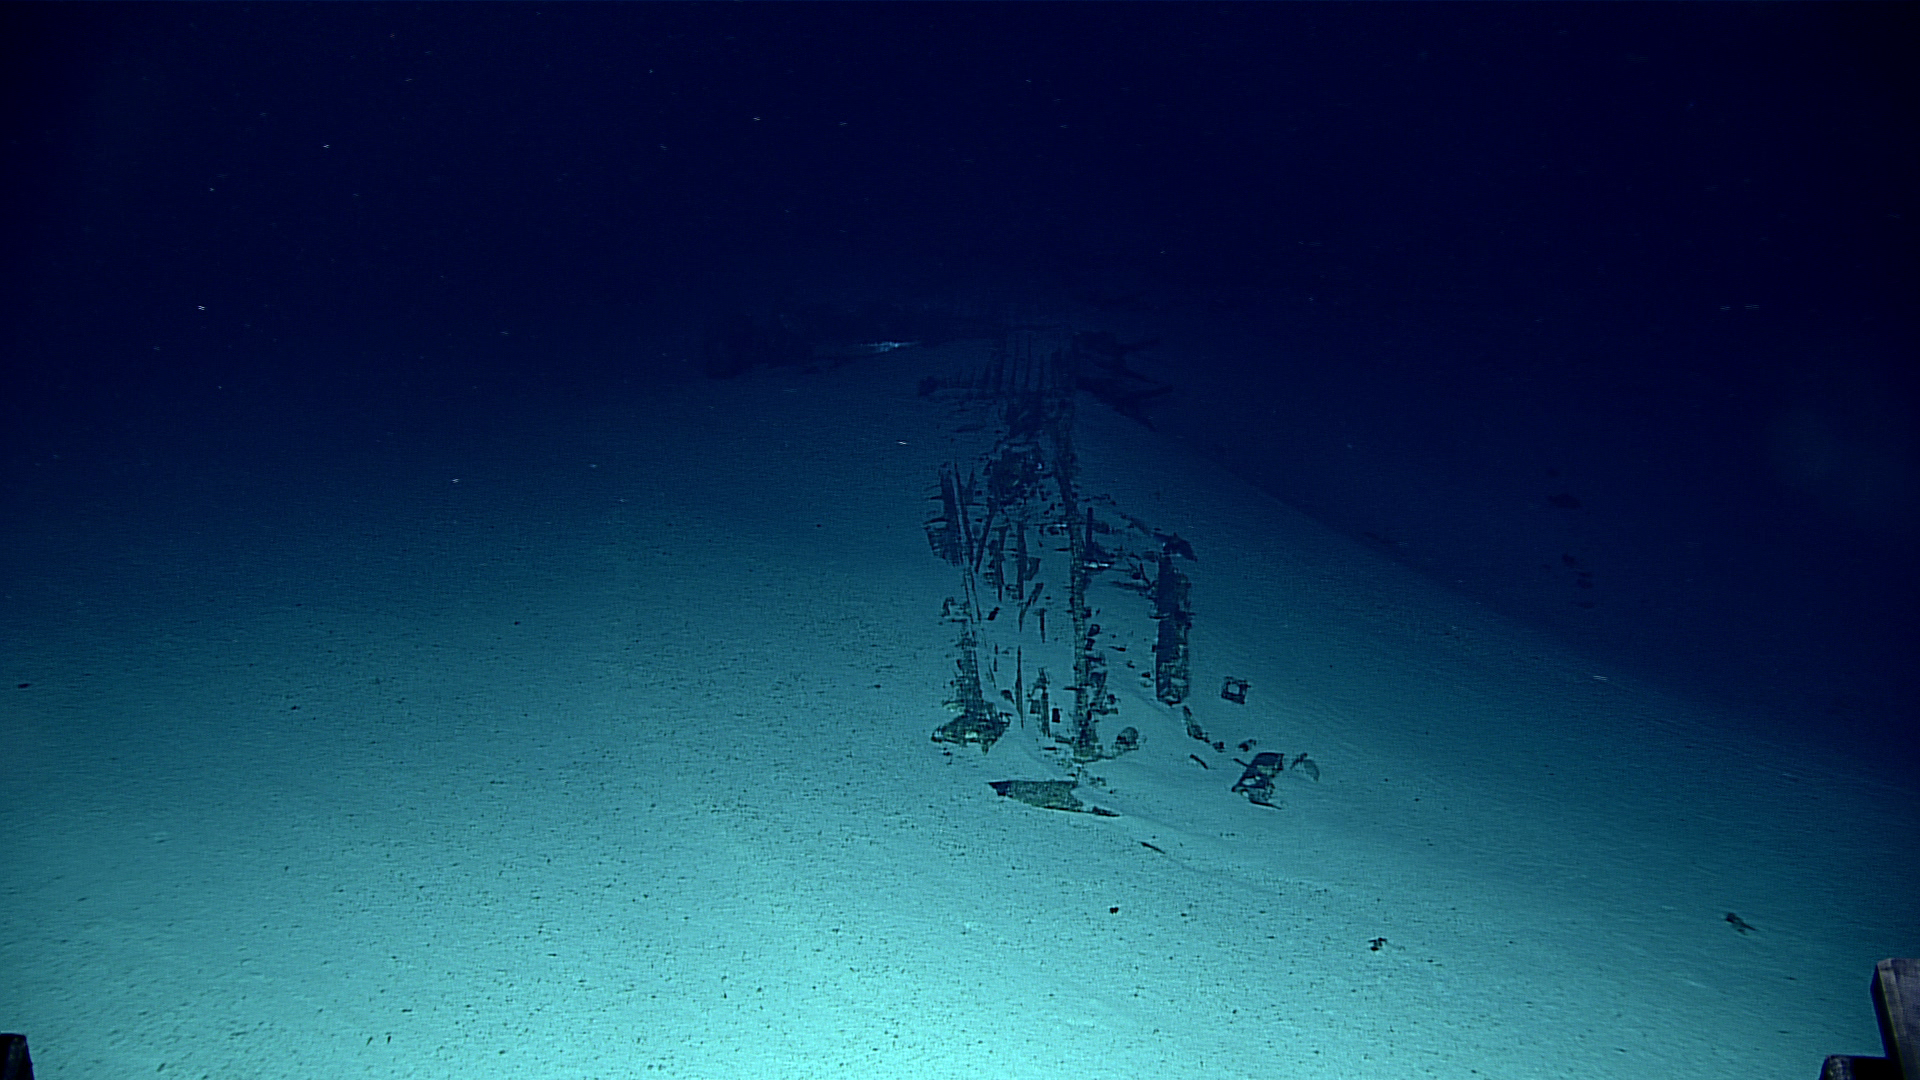
\includegraphics[width=\textwidth]{images/image_060000.png}
        \caption{Frame 60000.}
        \label{fig:ex1605l3_dive22_approaching_wing_begin}
    \end{subfigure}
    \begin{subfigure}[b]{0.48\textwidth}
        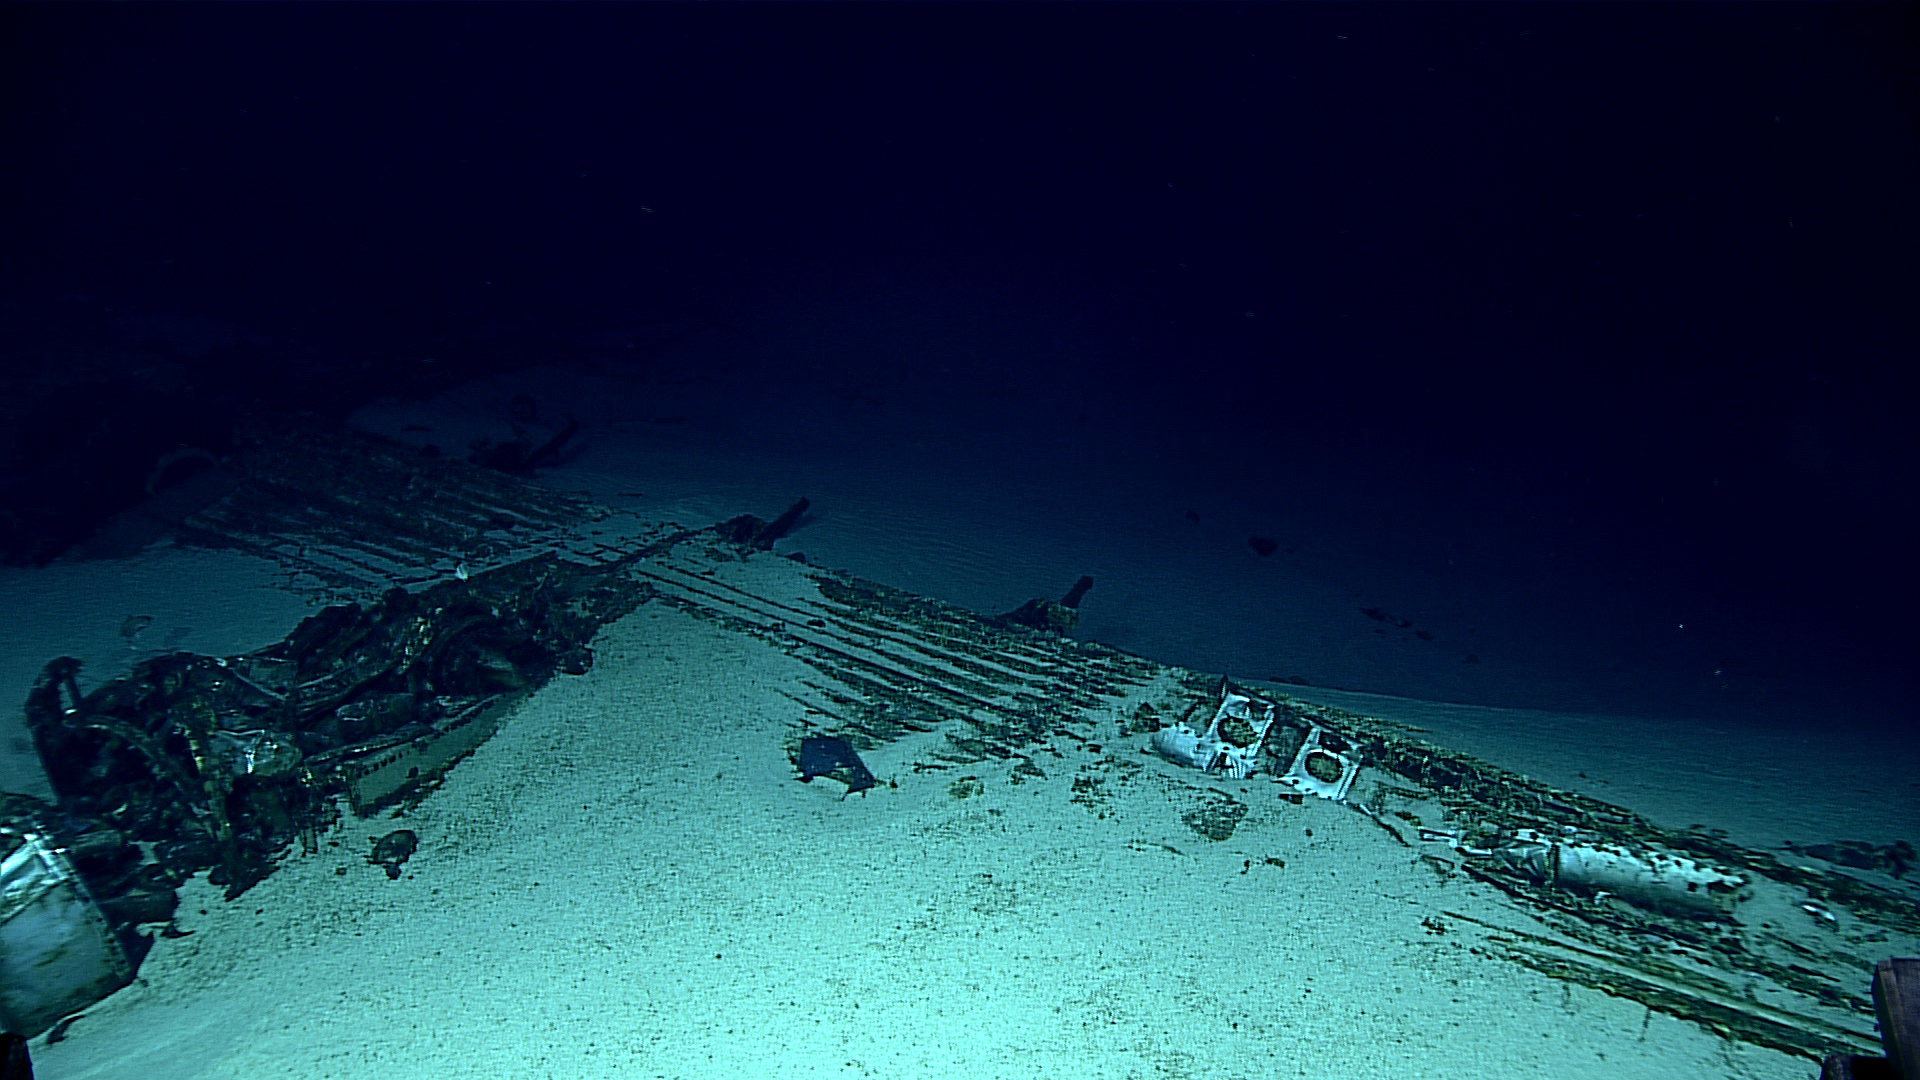
\includegraphics[width=\textwidth]{images/image_063400.png}
        \caption{Frame 63400.}
        \label{fig:ex1605l3_dive22_approaching_wing_end}
    \end{subfigure}
    \caption{First and last images in ``approaching wing'' segment within dive EX1605L3\_DIVE22.}
\end{figure}

\begin{figure}[p]
    \centering
    \begin{subfigure}[b]{0.48\textwidth}
        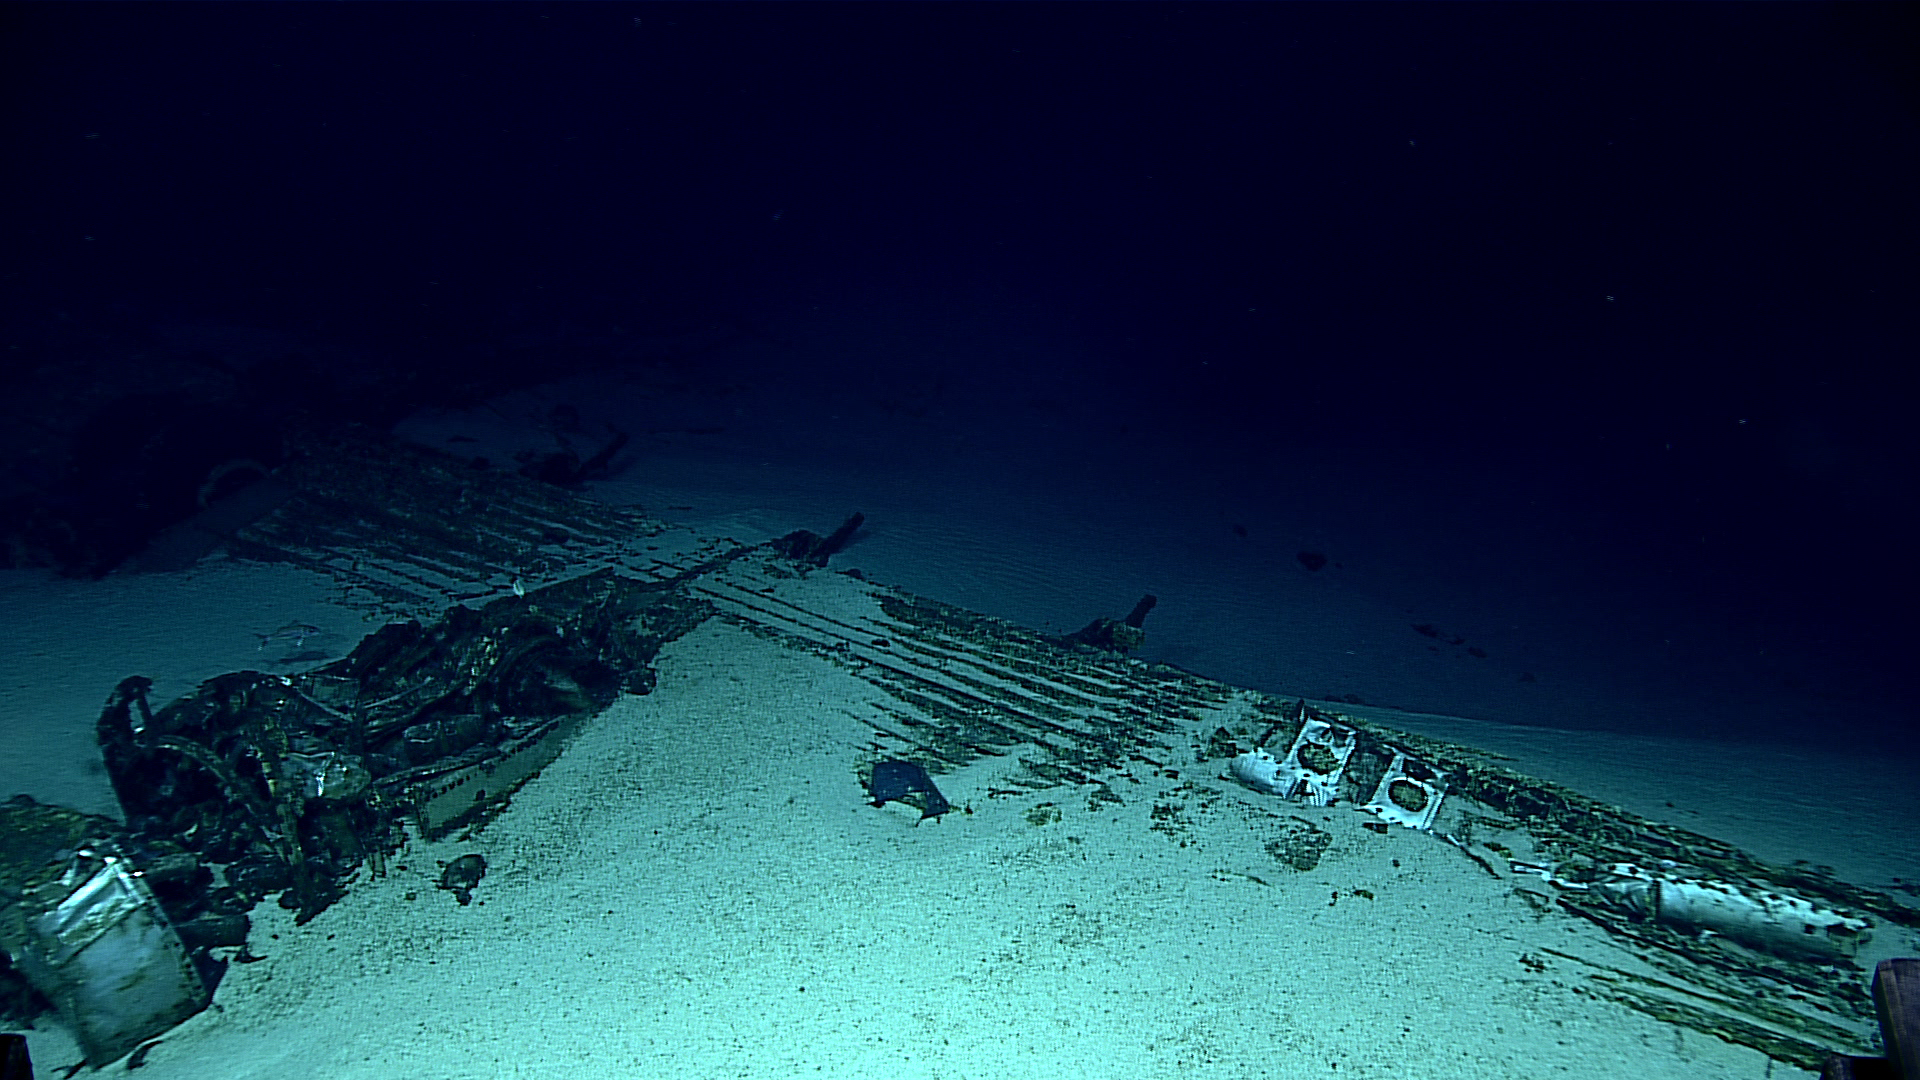
\includegraphics[width=\textwidth]{images/image_063500.png}
        \caption{Frame 63500.}
        \label{fig:ex1605l3_dive22_engine_one_begin}
    \end{subfigure}
    \begin{subfigure}[b]{0.48\textwidth}
        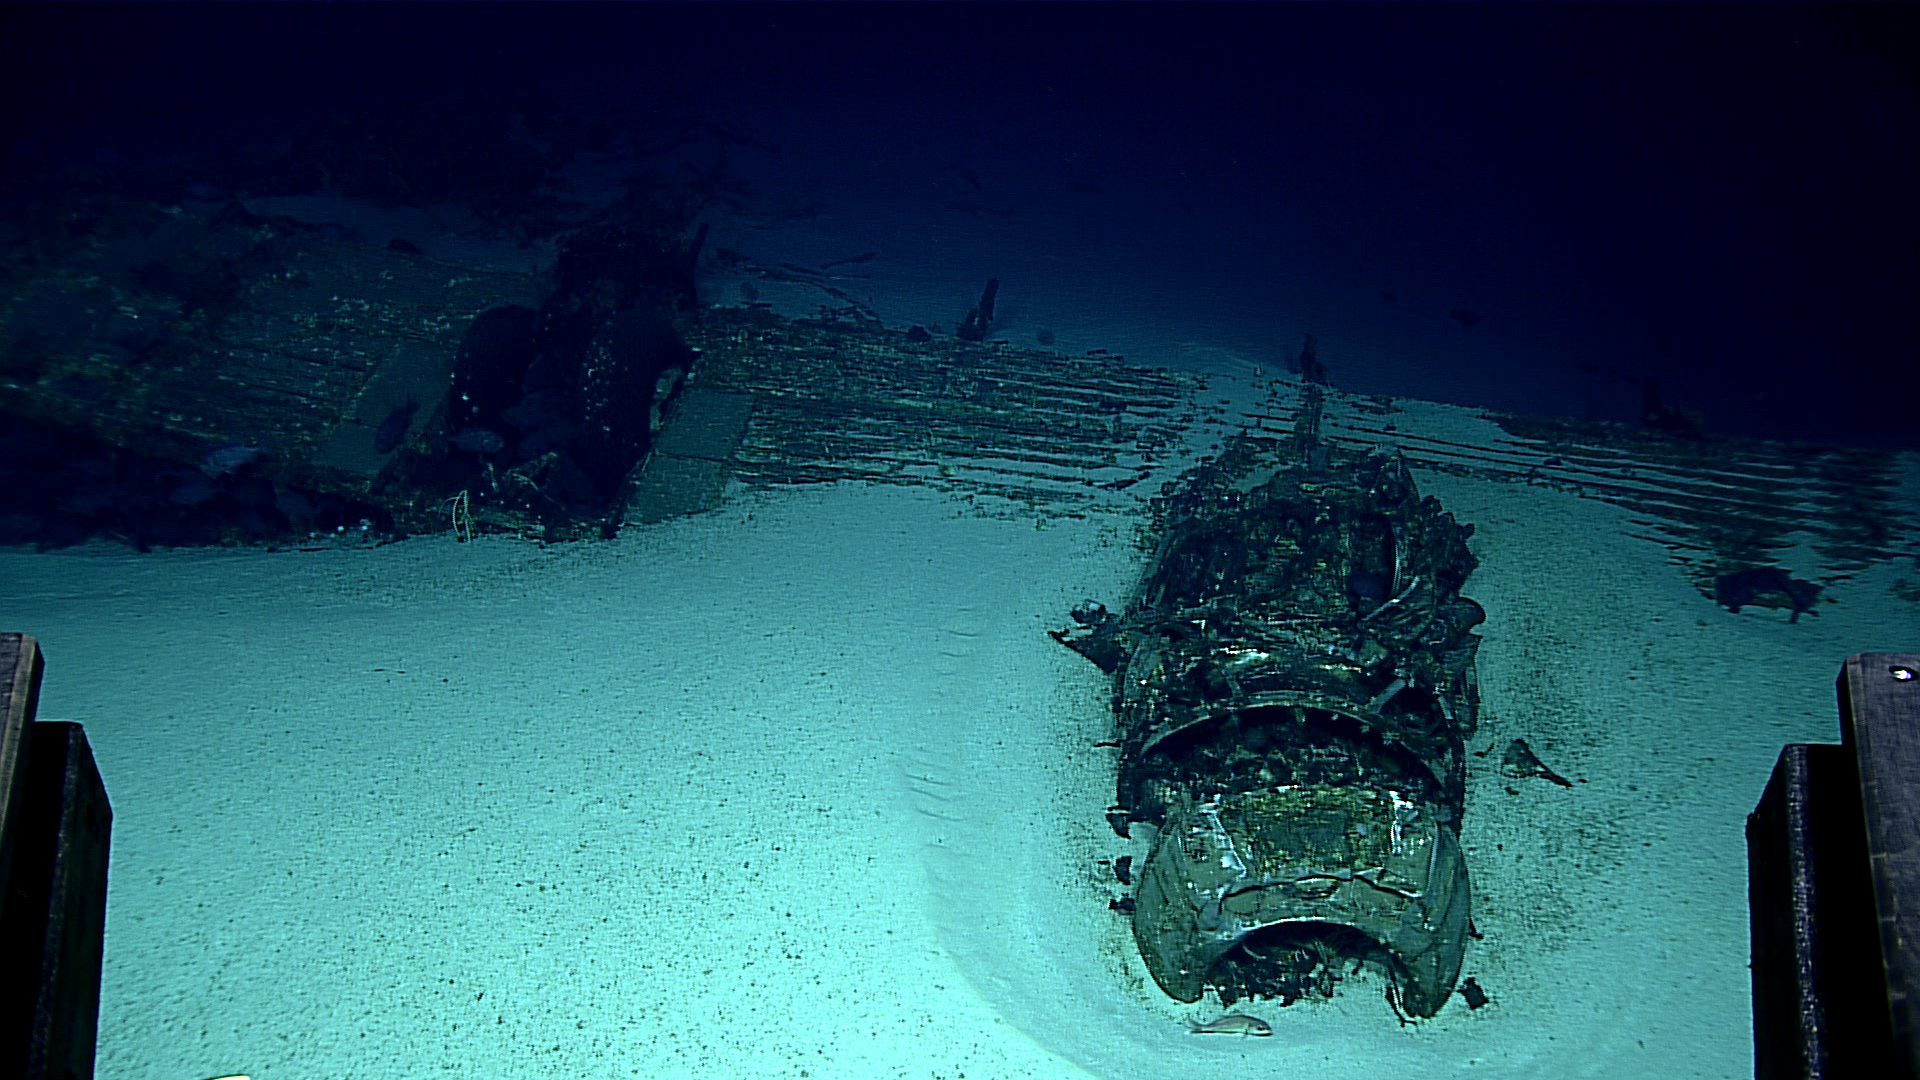
\includegraphics[width=\textwidth]{images/image_065900.png}
        \caption{Frame 65900.}
        \label{fig:ex1605l3_dive22_engine_one_end}
    \end{subfigure}
    \caption{First and last images in ``engine one'' segment within dive EX1605L3\_DIVE22.}
\end{figure}

\begin{figure}[p]
    \centering
    \begin{subfigure}[b]{0.48\textwidth}
        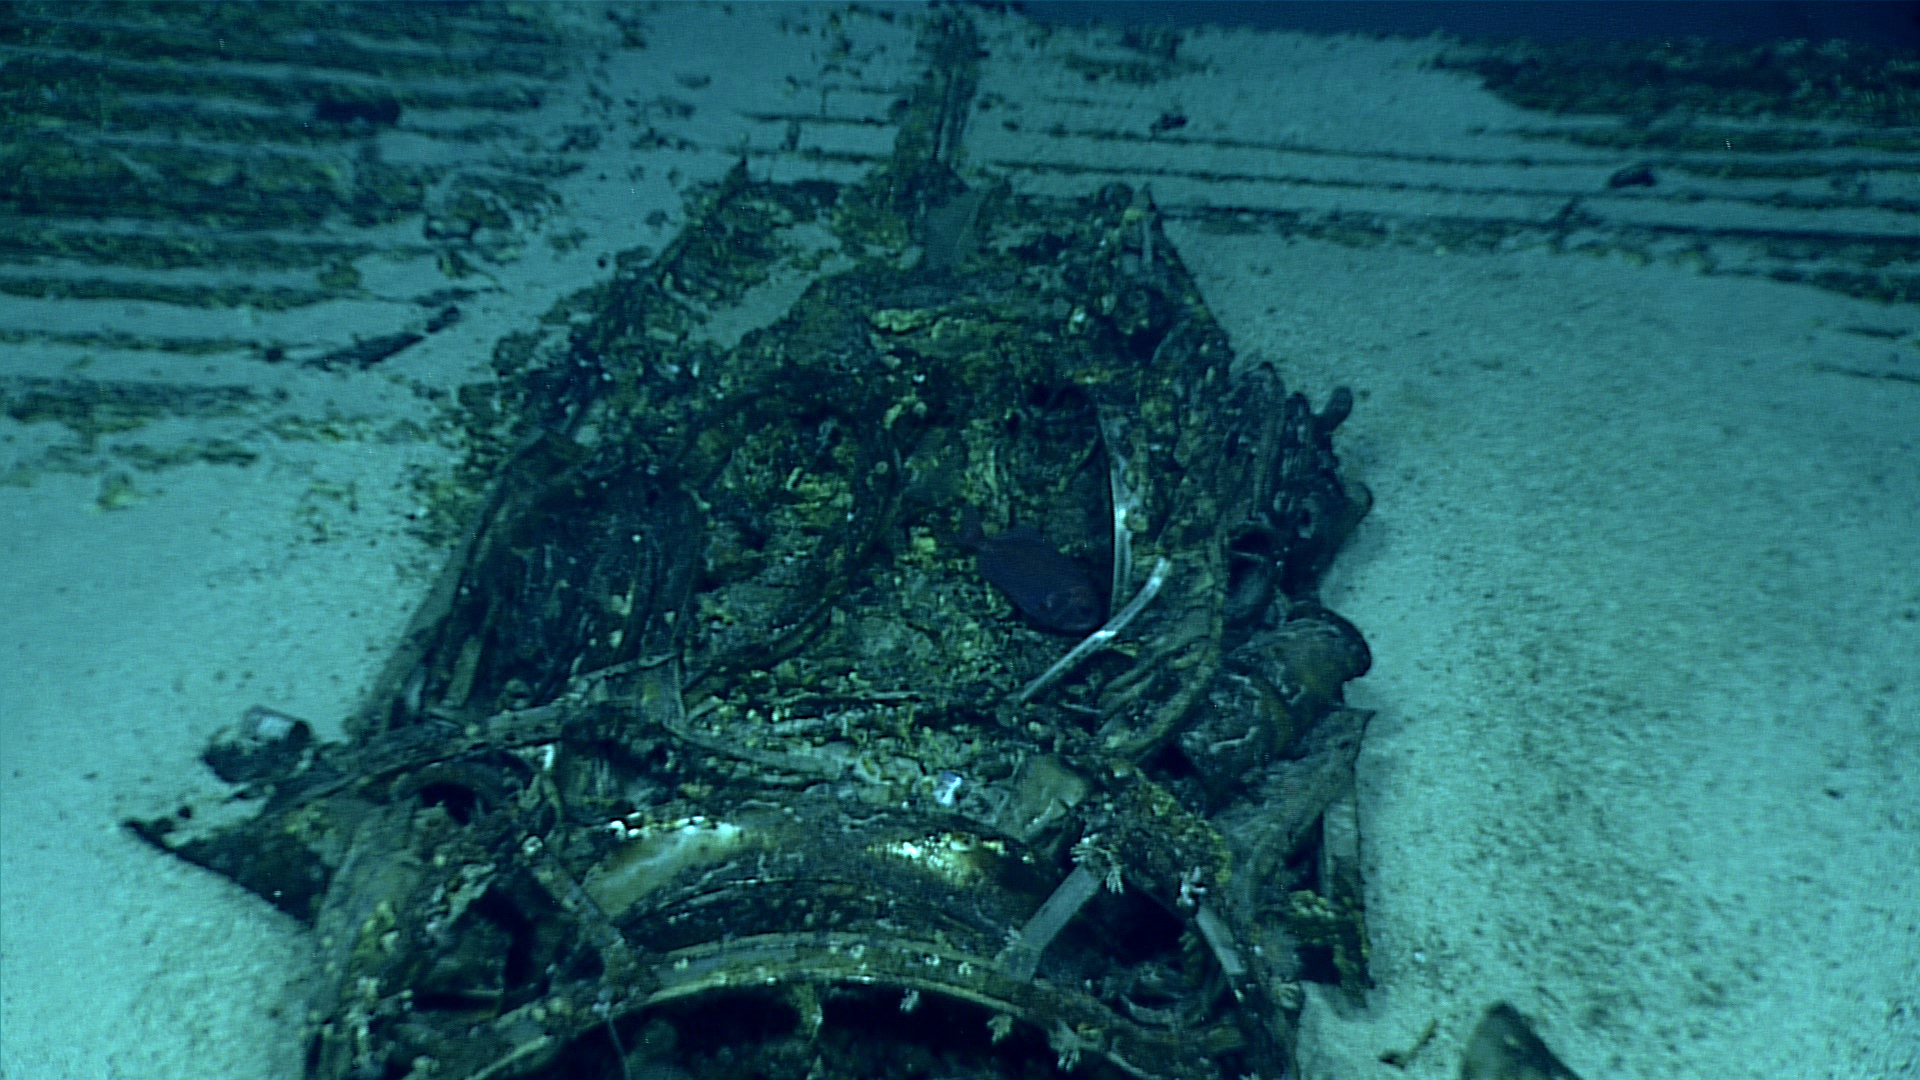
\includegraphics[width=\textwidth]{images/image_066400.png}
        \caption{Frame 66400.}
        \label{fig:ex1605l3_dive22_engine_detail_begin}
    \end{subfigure}
    \begin{subfigure}[b]{0.48\textwidth}
        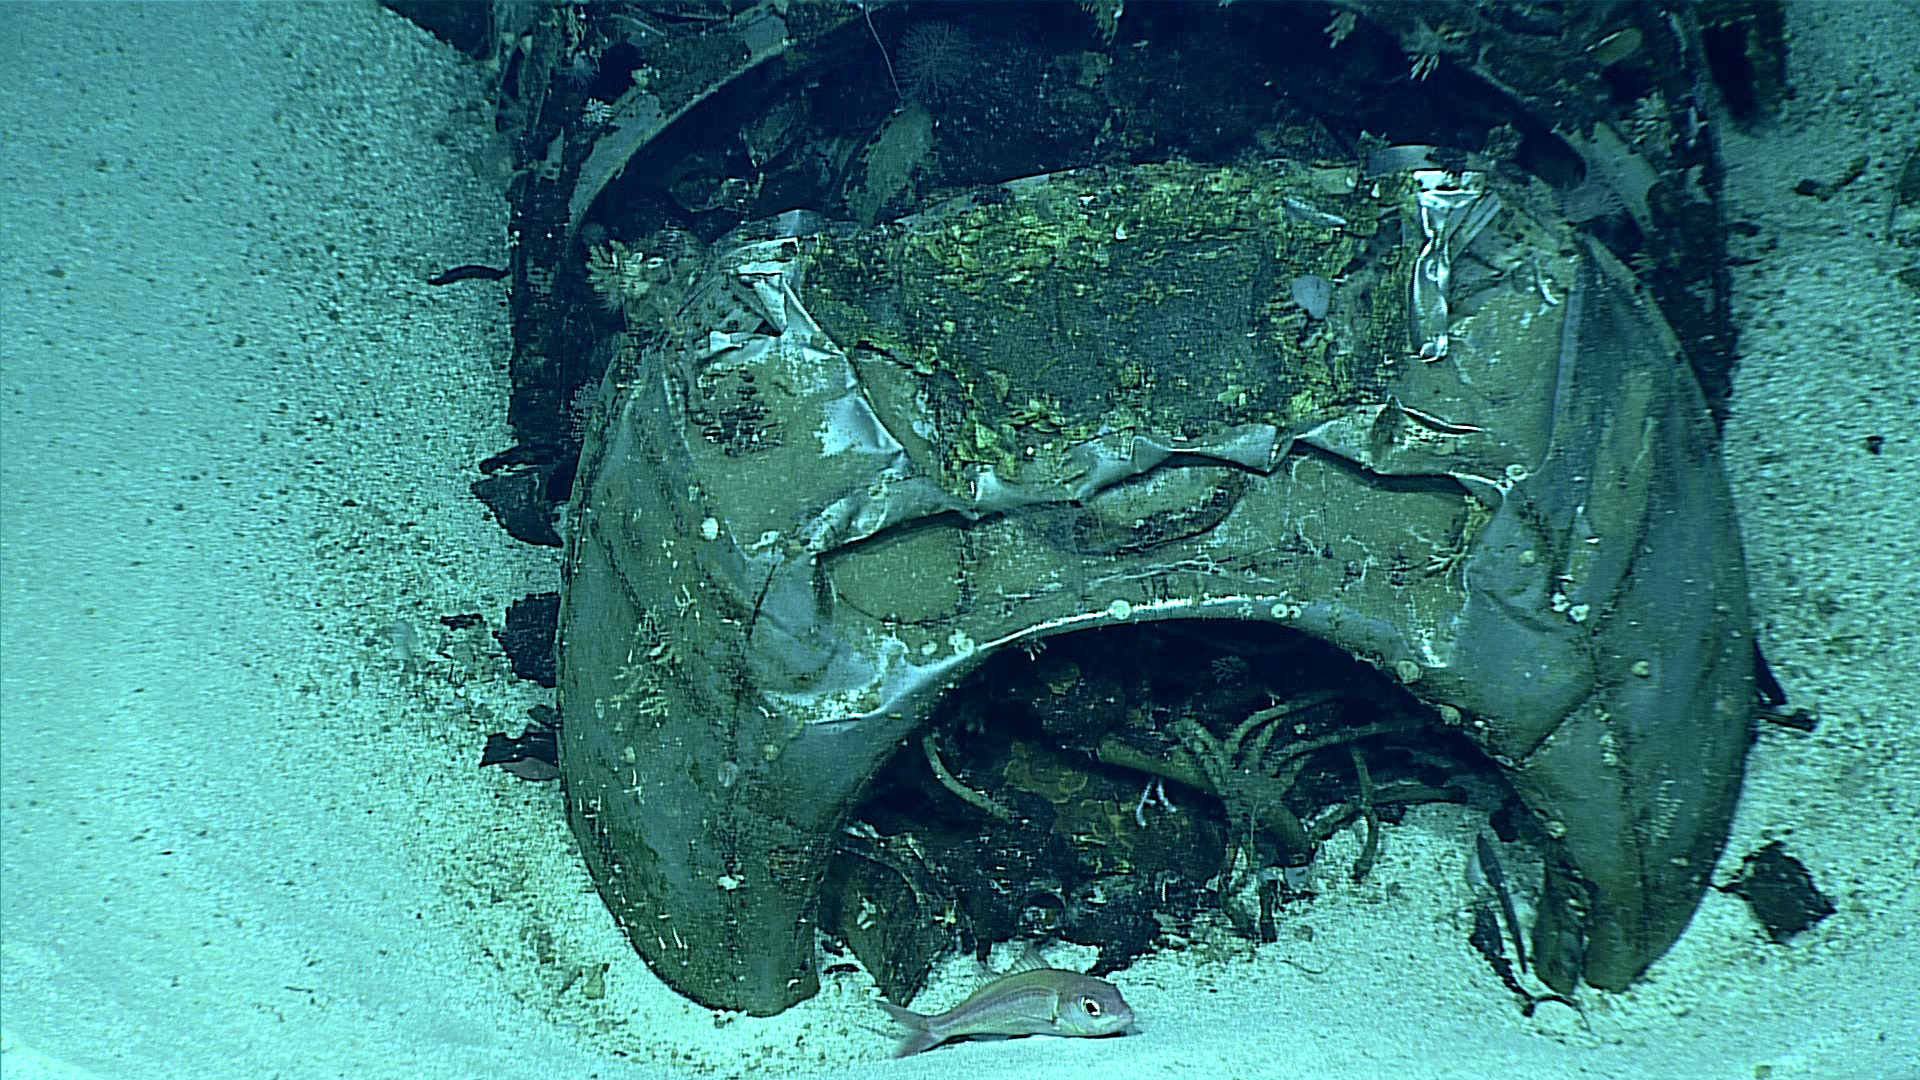
\includegraphics[width=\textwidth]{images/image_068900.png}
        \caption{Frame 68900.}
        \label{fig:ex1605l3_dive22_engine_detail_end}
    \end{subfigure}
    \caption{First and last images in ``engine detail'' segment within dive EX1605L3\_DIVE22.}
\end{figure}


\begin{figure}
    \centering
    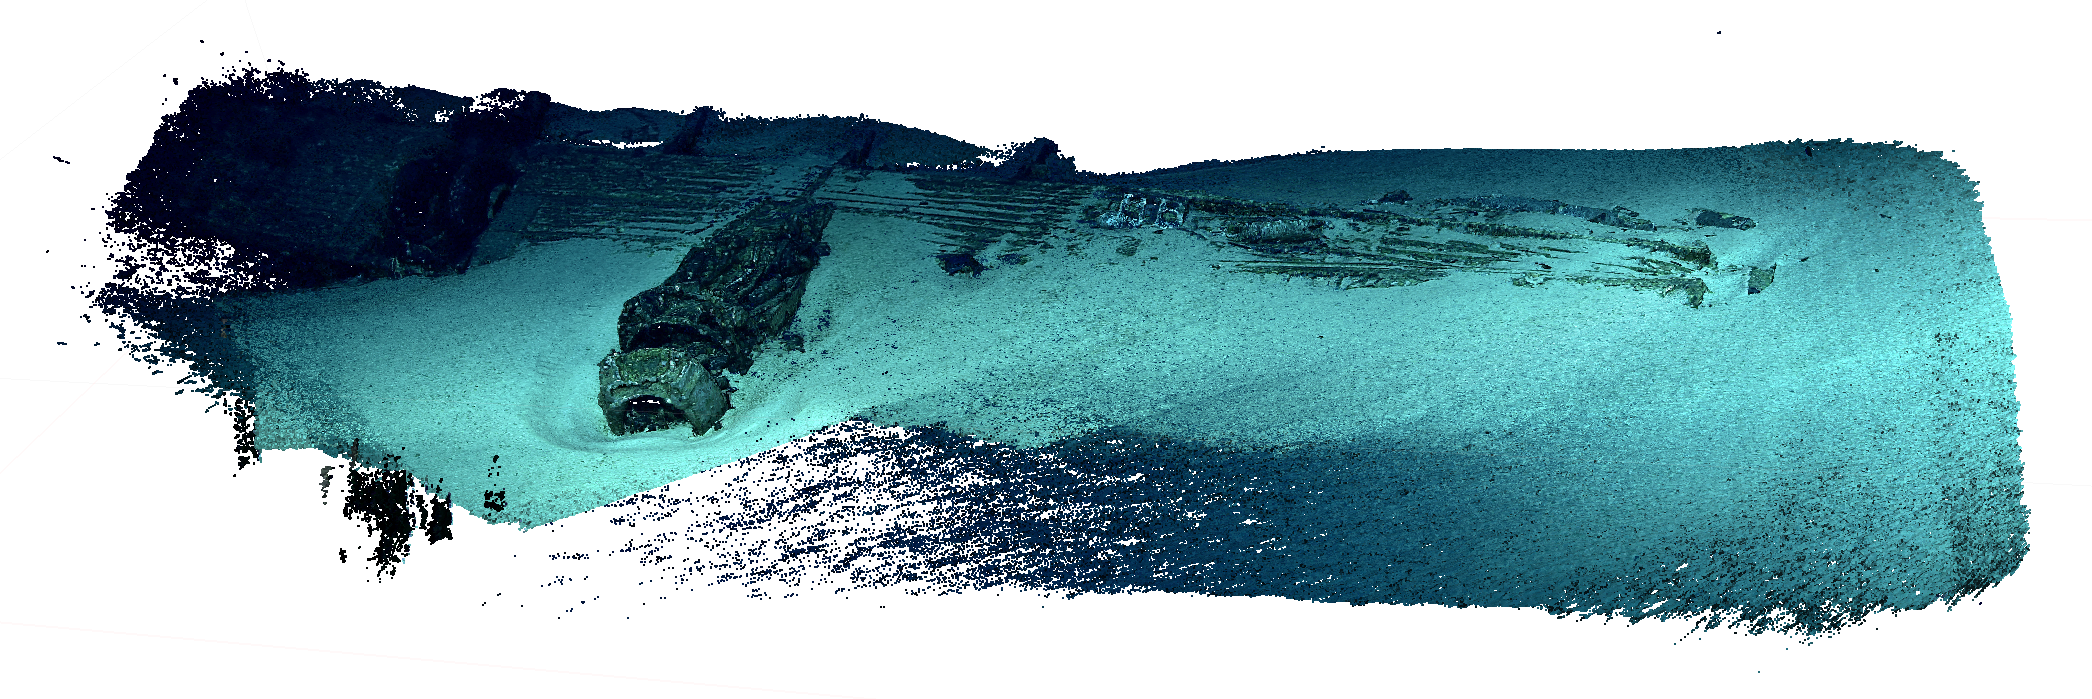
\includegraphics[width=0.95\textwidth]{images/approaching_wing_photoscan.png}
    \caption{Combined reconstruction of ``approaching wing'' and ``engine one'' segments of EX1605L3\_DIVE22.}
    \label{fig:ex1605l3_dive22_wing_photoscan}
\end{figure}

\begin{figure}
    \centering
    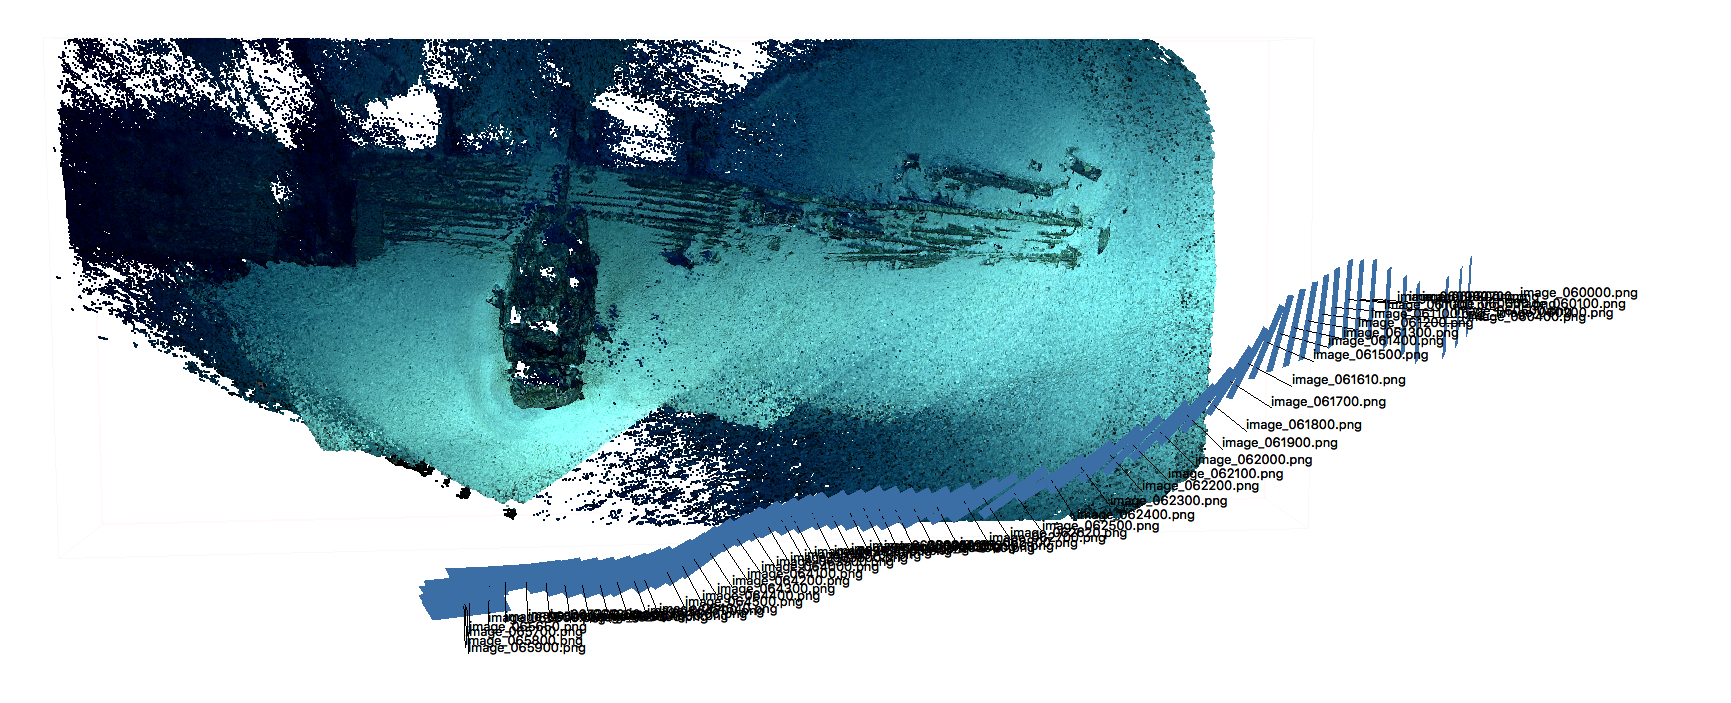
\includegraphics[width=0.95\textwidth]{images/approaching_wing_photoscan_trajectory.png}
    \caption{Reconstruction of ``approaching wing'' and ``engine one'' segments with overlaid trajectory.  ROV travels from right to left along leading edge of wing.   This segment concludes when ROV zooms in to examine engine nacelle seen at reconstruction center (see Figure \ref{fig:ex1605l3_dive22_engine_detail_photoscan}).}
    \label{fig:ex1605l3_dive22_wing_photoscan_trajectory}
\end{figure}

The ``approaching wing'' and ``engine one'' segments were processed independently in Photoscan then merged into a single model, as shown in Figures \ref{fig:ex1605l3_dive22_wing_photoscan} and \ref{fig:ex1605l3_dive22_wing_photoscan_trajectory}. 
The short ``engine detail'' section, during which the ROV was examining the nacelle of the number one engine, was also reconstructed independently as shown in Figure \ref{fig:ex1605l3_dive22_engine_detail_photoscan}.    This shows the fine detail possible from HD reconstruction, as well as the large data gaps which arise when viewing the subject from a single perspective.   This segment is particularly interesting in that it contains data from multiple camera zoom values, as shown in Figure \ref{fig:ex1605l3_dive22_engine_detail_photoscan_trajectory}.   While Photoscan assumes a constant focal length for all images from a given camerai, it compensates in this case by estimating that the camera location is progressively closer to the target.


\begin{figure}
    \centering
    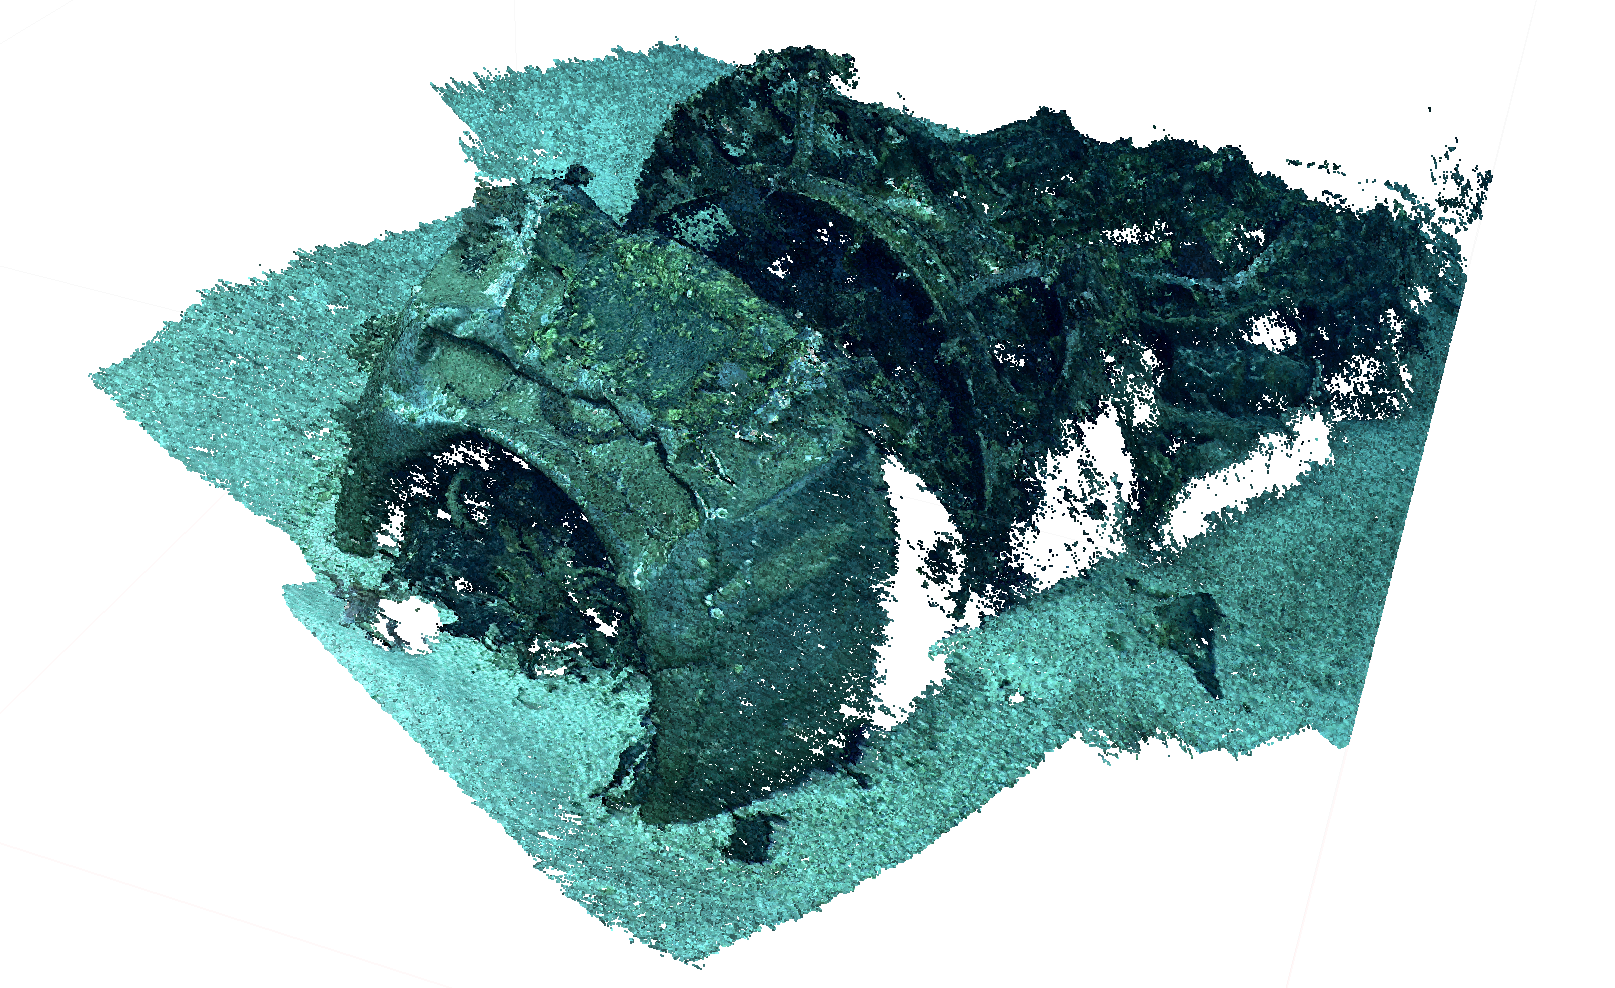
\includegraphics[width=0.95\textwidth]{images/engine_detail_photoscan.png}
    \caption{Reconstruction of ``engine detail'' segment from EX1605L3\_DIVE22.}
    \label{fig:ex1605l3_dive22_engine_detail_photoscan}
\end{figure}

\begin{figure}
    \centering
    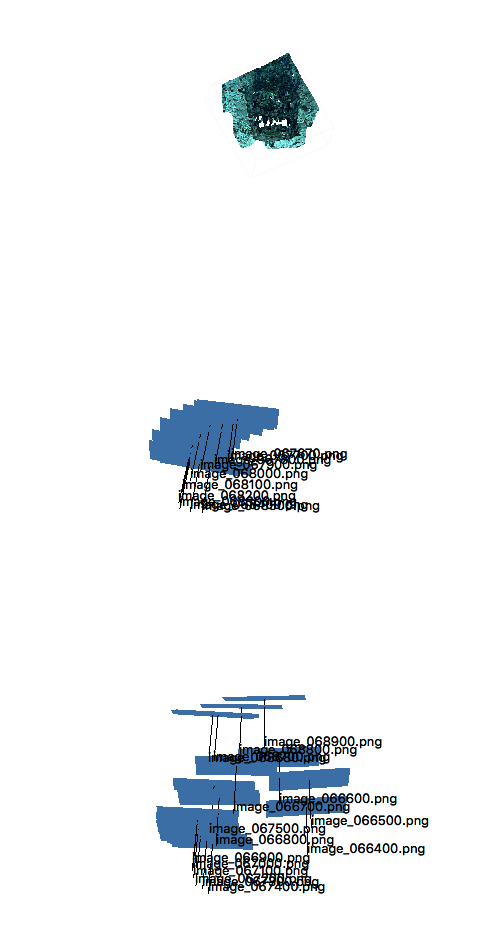
\includegraphics[height=0.9\textheight]{images/engine_detail_photoscan_trajectory.png}
    \caption{Estimated camera positions from of ``engine detail'' segment.  Model is shown at top.  The image clusters represent Photoscan's compensation for multiple states of camera zoom.}
    \label{fig:ex1605l3_dive22_engine_detail_photoscan_trajectory}
\end{figure}


\subsubsection{Realtime Reconstruction}

Whereas commercial products exist for post-processed reconstruction, realtime reconstruction remains an area of intensive academic research.   While many realtime reconstruction, or simultaneous localization and mapping (SLAM), systems have been detailed in the literature, there has been little convergence towards a set of commonly used tools.   This project started with the codebase for Large Scale Direct Simultaneous Localization and Mapping (LSD-SLAM), the product of Dr. Jakob Engel's PhD research at the Technical University of Munich \cite{engel2014lsd}.   Dr. Engels has released the LSD-SLAM code, along with several sample datasets, under an open source license allowing continued development after his completion of his degree.   As of the start of the project, LSD-SLAM was seen as one of the more accessible, better structured open source SLAM tools, with the understanding that any academically-based reconstruction tools might require intensive modification to accommodate the domain-specific challenges of this ROV imagery.

LSD-SLAM implements a modular system architecture in which the four primary tasks: tracking, local mapping, global mapping, and optimization, are segregated into discrete threads, allowing each task to operate asynchronously and in a prioritized manner, with the majority of CPU time reserved for realtime operations of tracking and local mapping.   As with many other realtime reconstruction algorithms, the core data structure in LSD-SLAM is a keyframe, which stores a particular image from the incoming video stream along with an estimated depth for a subset of that frame's pixels.   As new frames arrive, the tracking thread uses an optical-flow-based technique to estimate the camera pose of the current frame relative to the current keyframe.  This pose information is available immediately as an estimate of the current camera position for e.g closed loop control by a higher-level navigation process.  The mapping thread then uses the stereo baseline implied by that camera pose to update the estimated pixel depths for each of the current keyframe's pixels.   As a single keyframe is likely to match multiple subsequent frames, heuristics are used to ensure robust fusion of those depth estimates to update the depth map.

When the current frame is beyond a particular threshold in attitude or position from the previous keyframe, it is promoted to be the next keyframe.  Its depth map is initialized by projecting the previous keyframe's depth map into its frame of reference using the estimated inter-frame pose, and the processing continues with incoming frames matched against the new keyframe.  Compared to the number of images in the video stream, relatively few keyframes are retained, decreasing the overall data size.   Due to the keyframe selection mechanism, these keyframes are distributed spatially, rather than temporally, ensuring data model growth is proportional to area coverage, not time of exploration. 

Each keyframe is linked to its predecessor by the inter-frame pose at the time of its selection, forming a geometric constraint between the two keyframes.   Asynchronous to, and at a lower priority to the mapping/tracking processes, the global mapping task searches for image matches between non-sequential keyframes, looking to develop the so-called ``cross-tie'' geometric constraints which occur when a scene is visited multiple times within a single mapping mission.   If found, these cross-ties contribute additional geometric constraints between the two keyframes.     Finally, a global optimization thread, operating at the lowest priority of the four tasks, optimizes the full, mission-wide set of inter-keyframe geometric constraints, updating the pose of all keyframes.   

LSD-SLAM proved to be a powerful basis for developing a SLAM application, but also exceptionally brittle and difficult to modify.  Seemingly minor code changes would result in the software failing to function, and the overall software size and complexity made it very difficult to implement benchmarking or unit testing procedures to ensure code functionality while continuing development.   As a result, the original LSD-SLAM codebase required significant refactoring to be made usable.  The resulting version of LSD-SLAM is significantly more maintainable and produces identical results against the sample datasets provided by Dr. Engels \cite{lsdslam}.   However, the current version does not correctly generate reconstructions over the ROV video segments identified above.  As shown in Figure \ref{fig:lsd_slam_engine}, the LSD-SLAM software correctly imports and processes images from the video segments, however the resulting reprojected depth maps are essentially flat.   This is assumed to be a bug in LSD-SLAM rather than an issue with the underlying data, although it is possible that the particular video segments selected are challenging to process in a realtime manner.

\begin{figure}
    \centering
    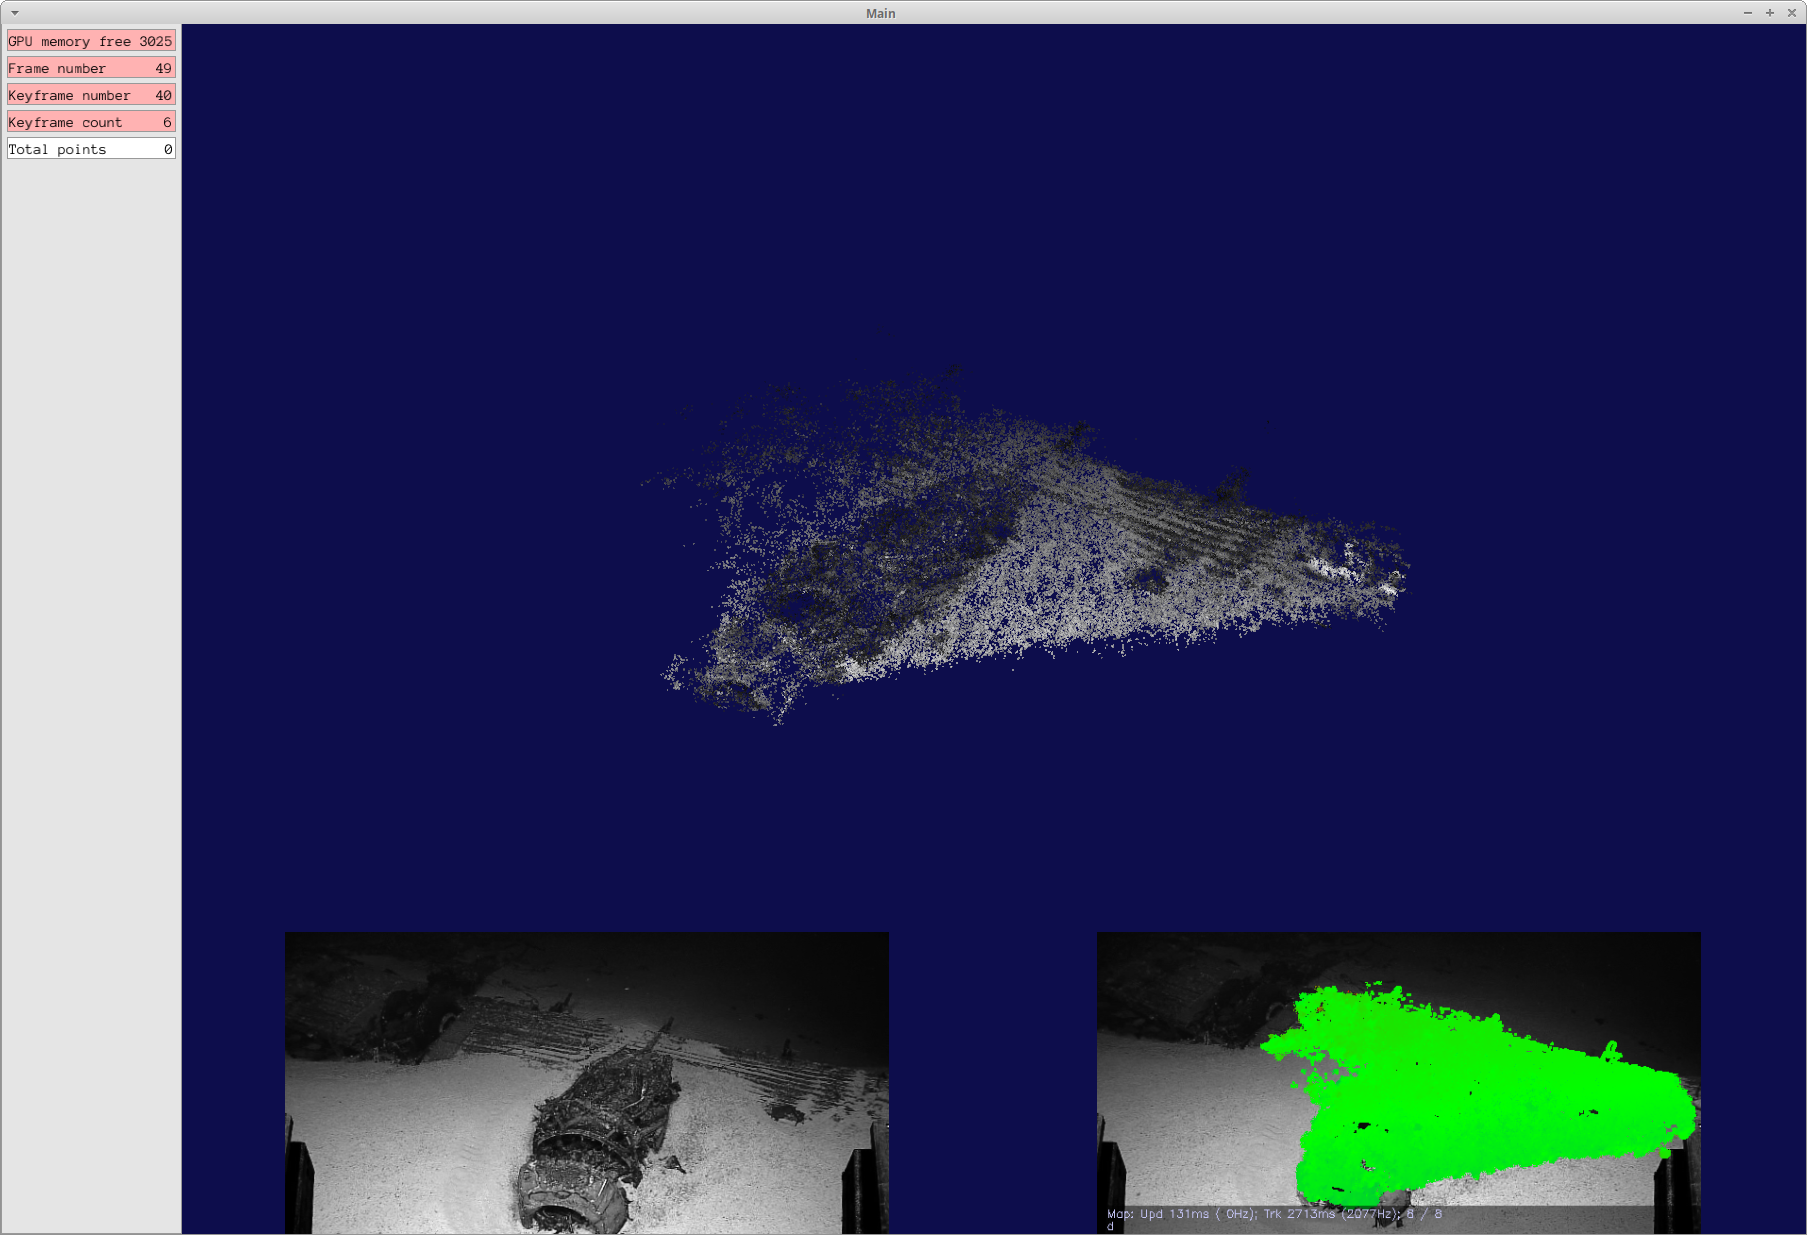
\includegraphics[width=\textwidth]{images/lsd_slam_engine_two.png}
    \caption{LSD-SLAM software display while processing ``engine one'' dataset.    Current input image is shown on lower left, and input image with color-mapped depth on right.   Full point cloud to this point is shown above.  As shown in this image, LSD-SLAM has correctly projected multiple images into point cloud space, however it has not correctly developed a realistic depth model from those images.} 
    \label{fig:lsd_slam_engine}
\end{figure}

\begin{figure}
    \centering
    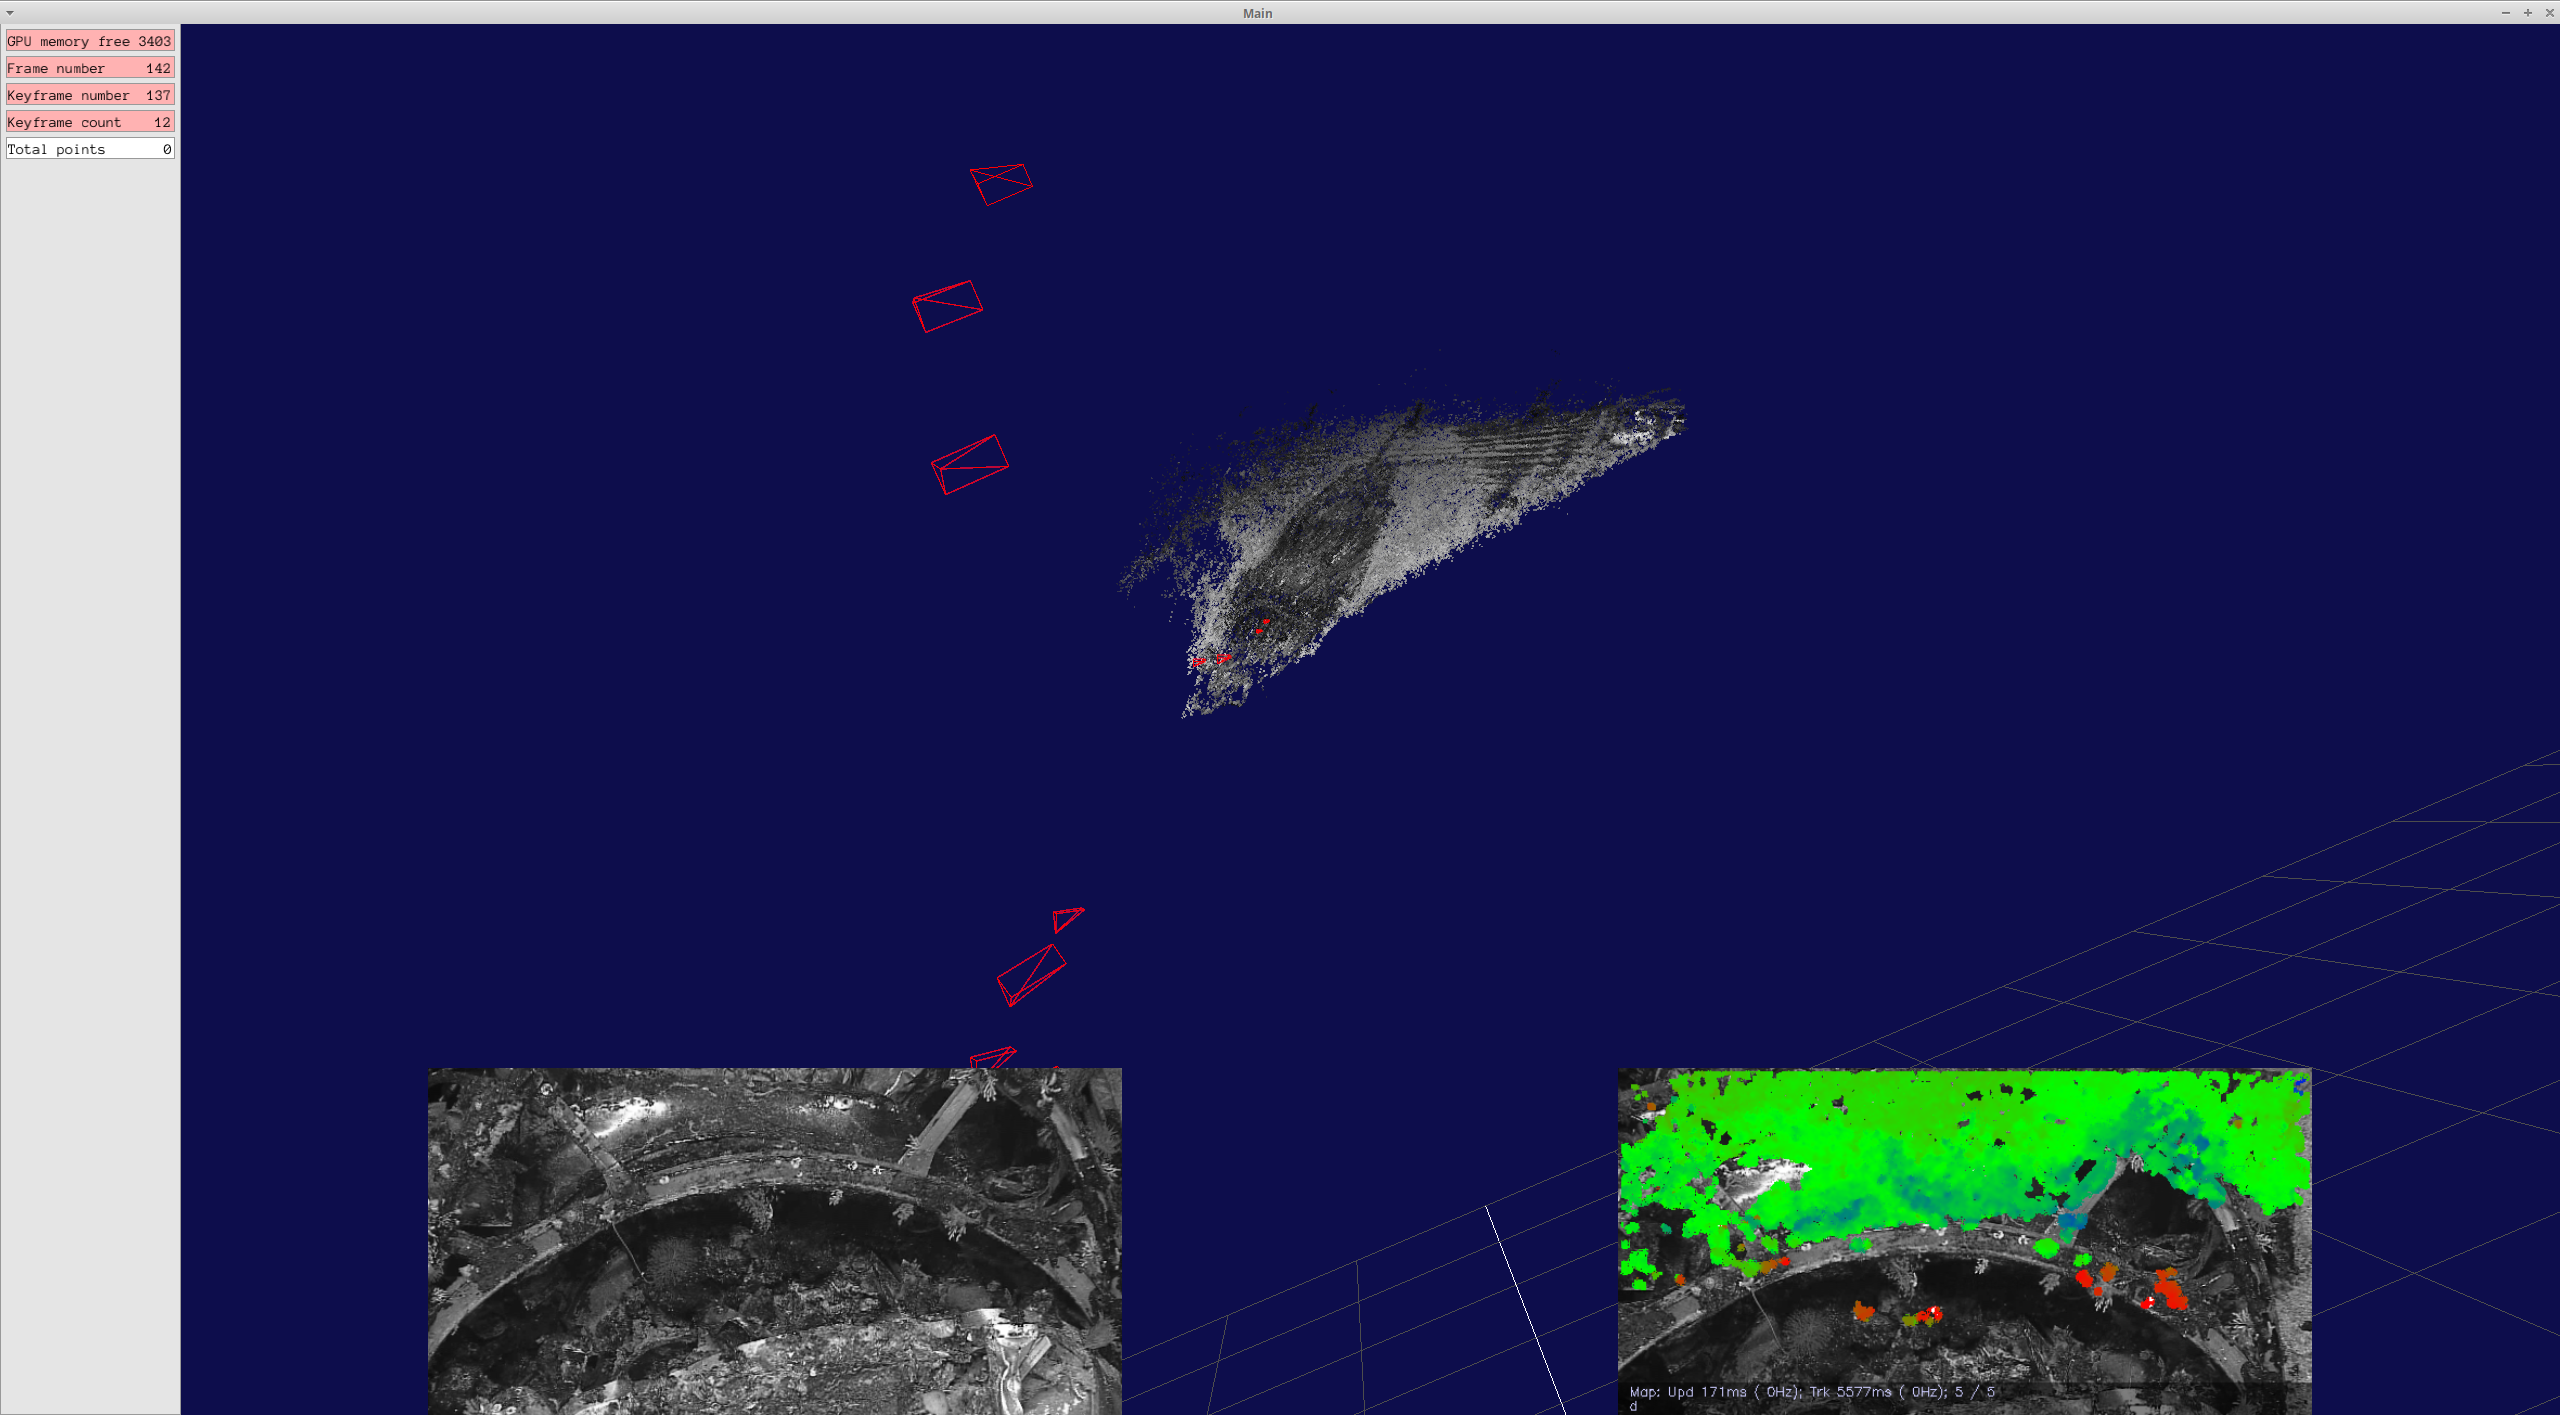
\includegraphics[width=\textwidth]{images/lsd_slam_engine.png}
    \caption{LSD-SLAM software display after continued processing of ``engine one'' dataset.  Red pyramids represent keyframe poses.   Note this image occurs after the camera has started to zoom in from ``engine one'' to ``engine detail.''  LSD-SLAM has continued to track throughout the transition as shown by smaller poses approaching the front of engine.}
    \label{fig:lsd_slam_engine_detail}
\end{figure}


 
 
\subsection{ROV mission planning and execution for 3D reconstruction}

The disparity in success between the post-processed and realtime reconstructions provides an ideal segue into the third project objective, evaluating the suitability of the D2 video as it is currently collected for 3D reconstruction.  The results from the post-processed reconstruction clearly show that the HD science camera video is suitable for 3D reconstruction.  In preparation for the project, three potential data error sources were considered as prime candidates for reducing reconstruction success:   occlusion from the ROV superstructure or manipulator; the aforementioned variable scene appearance due to fading and color shifting with distance from the light source; and unmodelled camera motion (i.e., the fact that the camera operator freely moves the camera to meet science objectives and the fact that motion is not otherwise recorded in the metadata).     The first was of limited concern in the sample data sets.    The field of view from the science camera is almost completely unoccluded in the provided video, as none of the segments feature use of the ROV manipulator.   A small portion of the retracted science skid is visible when the camera is tilted downward, however Photoscan provides a simple binary masking tool which allows exclusion of portions of each image.   Occlusion would be of far greater concern if a mission featured active manipulation, and it's fair to say that future missions should segregate periods of observation from periods of manipulation.

Lighting effects had surprisingly little impact on the reconstruction process.  As noted previously, the variable coloring of more distant objects impacts the coloring of the final point cloud but does not appear to have affected the point cloud geometry itself.   Assuming there are no gross errors in the resulting geometry, this is a testament to the robustness of the point correspondence algorithms within Photoscan.  

Camera pan and tilt motion was also of little consequence.  The reconstruction is geometrically tied to the camera's pose and camera tilt and yaw simply appeared as changes in image position.  As a result, the image positions from Photoscan reflect \textit{camera} positions, not \textit{ROV} positions, however if there were a desirable output (for example to use the reconstruction for navigation), the pose offset between the ROV's inertial frame and the camera's frame could be measured and the ROV pose calculated.

By far the most consequential video artifact is the use of optical zoom.   Neither Photoscan nor LSD-SLAM are designed to correctly account for changes in the camera's focal length, however both appear to compensate correctly by introducing an artificial change in the camera-to-object distance (as in Figures \ref{fig:ex1605l3_dive22_engine_detail_photoscan_trajectory} and \ref{fig:lsd_slam_engine_detail}).   While this introduces a gross error into the estimated trajectory, it maintains the quality of the resulting point cloud.    A greater problem, demonstrated by the transition from ``hillside'' to ``top of slope'' is the need for sequences of images with recognizable overlap to form robust correspondences.  With high-rate video this requirement is met by default, bar either blurring or turbidity, and when post-processing, the set of images used for the reconstruction can be adaptively curated to maintain good image overlap independent of vehicle speed, selecting images at long intervals when the vehicle is moving slowly and progressively more frequently when the vehicle is moving quickly.

This dynamic is disrupted by the reduction in field of view seen in the three segments from EX1605L3\_DIVE4.    There is minimal or no overlap between the final wide-angle images in ``hillside'' and the first wide-angle images in ``top of slope,'' and as the general trajectory in ``top of slope'' is upward and away from ``hillside'' there are no opportunities to match the two video sequences.   As such the two reconstructions are disjoint and cannot be merged.    It should be possible to maintain an estimate of vehicle trajectory throughout the 3-minute zoomed-in ``upslope'' segment, however, even if the three segments could be joined, the underlying geometry would be suspect at best, with the two large-scale segments joined through the relatively few geometric constraints in the ``neck'' of ``upslope.'' 

The role of the video properties on the failure of LSD-SLAM is harder to diagnose.   A large portion of the deficiencies of LSD-SLAM can be assigned to its status as research-grade or experimental software which simply could not be brought to an appropriate level of maturity within the time frame of this project.    Beyond that, it is less clear if the ROV video was inherently more difficult to process in realtime than in post-processing.

In conclusion, video from the D2 is certainly suitable for reconstruction.   The success of the post-processed results indicates that the underlying video data is of sufficient quality to produce high-grade photo-quality reconstructions, even from mission segments where photogrammetric data collection is not the explicit mission goal.   That said, reconstruction quality can be directly improved by the same mission planning factors that improve terrestrial photogrammetry:   ensuring image overlap, capturing redundant imagery, and ensuring coverage.   The value in the former is highlighted by the issues connecting the ``hillside'' and ``top of slope'' segments, where the issue is not the period of close examination, but the vehicle motion during that period which eliminates overlap before and after the gap.   This also highlights the importance of multiple crossing or re-viewings in developing robust reconstructions.   Both the ``hillside'' and ``top of slope'' segments, while featuring high image overlap, are essentially linear transects, with no repeated viewings of areas of interest.   Small errors in geometric alignment between images can propagate, leading to gross errors at the end of each segment.   When metric accuracy is critical, it is critical to view objects of interest from multiple perspectives.   

The question of coverage is also relevant in a scenario which was not present in the data shown here: when the ROV is not able to continuously track an object but instead must ``look away'' into open water.  As an example, ``top of slope'' concludes as the ROV ascends vertically and the slope moves out of range of the lights.     Were the ROV to then descend again to bring the slope back into sight, there is no guarantee that the reconstruction could bridge that gap.   For post-processed reconstruction, if the scene after returning to the slope has sufficient image overlap with a previous scene, the operator could select appropriate images to ``stitch'' images from before and after the gap into a single model.    For realtime, however, the system would need to be robustness enough to track the ROV's motion while ascending, recognize that it was unable to maintain track as the ROV moved into the open water, then correctly jump back to a \textit{previous} keyframe, given only a limited geometric prior, when it re-entered its previous trajectory.  Such re-acquisition is an area of intensive research in the SLAM community and can be extremely challenging.    Such a scenario is of particular concern in the subsea because the blank open ocean represents such an omnipresent background.   In terrestrial applications, it is rare for there to be \textit{nothing} to look at and track, even if it is only background and not the scene of interest.

The second factor which advocates for explicitly planning of video collection for reconstruction is coverage.  As shown by all of the models in this project, photogrammetric reconstruction can only model portions of the scene which are actually observed.   Without explicit survey procedures designed to maximize coverage, it is very difficult for human operators to estimate data gaps.  Herein lies one of the true advantages of online reconstruction for ROV mission execution --- to provide feedback on the state of a reconstruction and ensure an appropriate level of coverage in subsequent post-processing.

% \subsubsection*{Inventory of activities (number of submersible dives, CTD, net tows, etc.)}

% \subsubsection*{Inventory of samples collected}

\subsubsection{Describe/list/append resulting publications, Web sites, presentations, etc.}

Project progress was documented at the website \url{https://noaa-oer16-3dreconstruction.github.io/public-www/}.    Links to relevant project data sets, including the input imagery for the video segments listed above are posted there.

%\subsubsection*{Location and status of data archive and/or sample storage, plan for public access, and final data inventory} 

%\subsubsection*{Notation of major changes/adjustments to previously submitted documents (e.g.    Quick Look Report, Semi-Annual Report, and/or Annual Report)}

\section{Evaluation}

\subsection{Accomplishments}

Of the three objectives discussed in the report introduction, post-processed reconstruction from archival D2 video was the most successful, with reconstruction demonstrated for a subset of relevant mission types.   The tools and procedures generated under this project provide a basis for repeatable, documented extraction of image sets from potentially very large, multi-file movie sets, increasing the transparency of the reconstruction process.   Despite the time investment, the second goal of realtime reconstruction was only partly successful.   There is no doubt the project team has a much more thorough knowledge of LSD-SLAM, and the current version of the software is more robust, more modifiable and more manageable than the original version produced by the Dr. Engels.  However as discussed previously, it is not mature enough to actually reconstruct the ROV video provided by NOAA.  Again, it is unclear to what degree this failure comes from the software --- either an inherent weakness in the LSD-SLAM concept, or more likely a bug introduced during the software re-engineering --- and to what degree it is due to a challenge arising from the ROV video itself.

\subsection{Expenditures}

The award and final budget expenditures are detailed below:

\begin{tabularx}{0.9\textwidth}{X|rrrr}
    & \textbf{Award} & \textbf{Expenditures} & \textbf{Expenditures} &  \\
    & \textbf{Amount} & \textbf{Year 1} & \textbf{Year 2} & \textbf{Balance} \\
    \hline\hline
    Salaries \& Wages & \$36,122.00 & \$36,653.27 & \$4,528.01 & (\$5,059.28) \\
    Staff Benefits & \$18,685.00 & \$19,718.06 & \$2,763.35 & (\$3,796.41) \\
    Travel & \$11,496.00 & \$251.83 & --- & \$11,244.17 \\
    Services & --- & --- & --- & --- \\
    Supplies & \$1,000.00 & \$1,241.86 & \$370.02 & (\$611.88) \\
    Equipment & --- & --- & --- & --- \\
    Other & \$21,537.00 & \$20,346.25 & \$2,436.36 & (\$1,245.61) \\
    Indirect Cost & \$16,880.00 & \$14,860.13 & \$1,918.57 & \$101.30 \\
     \\
    Total & \$105,720.00 & \$93,071.40 & \$12,016.31 & \$632.29 
\end{tabularx}

\vspace{12pt}
\noindent
As per the original award, the project expenditures were almost exclusively salary support for the project team.  The original proposal included a trip to rendezvous with the D2 at a port of call to perform an explicit calibration of the main science camera.  This proved to be both challenging to schedule and unnecessary as the intrinsic properties of the camera could be derived directly from the data.

\subsection{Next Steps}
\subsubsection*{Planned or expected reports (professional papers, presentations, etc.)}

A description of the project outcomes is in preparation for the 2019 IEEE/MTS Oceans conference to be held in Seattle in October 2019.

\subsubsection*{Brief description of need for additional work, if any (next project phase, new research questions, unaccomplished work, etc.)}

Perhaps more than the project team hoped, this project only served as a first step into the exploration of 3D reconstruction from ROV video.  Results with Photoscan were very encouraging and will drive a further conversation on the role of 3D models as a value-added output from ocean exploration, either as a synthesis product for public outreach (a ``compelling visual'') or as a secondary data product.     

The issues with reconstructing the ROV video with LSD-SLAM should not overshadow the investment made in learning and improving the underlying system.   LSD-SLAM has been shown to be a successful and usable SLAM system, but as might be expected with a complex algorithmic system, it suffers from a much steeper learning curve than initially predicted.   
From this point, there are a number of potential avenues for future investigation:

\begin{enumerate}
    \item Achieving realtime reconstruction of D2 video using LSD-SLAM.   The project staff firmly believe LSD-SLAM is closer to being a robust and usable product than at project inception, and that the issues shown here are due to minor bugs rather than major structural faults.   As it stands, the LSD-SLAM code is better engineered, higher performance and more robust than the original codebase, and further research on other sponsored projects will contribute further to its development.   Having the D2 ROV videos on hand provides an ideal set of test images for further testing and development.
    
    \item Best practices in ROV mission planning for reconstruction.   The next logical step is to invert the original value proposition of this project.   If the generation of a 3D model is the explicit goal of a portion of an ROV dive --- a scenario which is easy to imagine for many archaeological missions --- how does is this translatated into the actions of the ROV crew while on the dive?   At a minimum, designating periods of explicit, structured, fixed-focal-length survey over the area of interest, capturing multiple views from varying perspectives, is critical to maximize model quality.  To state it another way, good models can be generated from many videos, but full coverage requires conscious mission design.
    
    \item Robustness in turbid waters.  The reconstructions shown here are successful in no small part because the video is taken in deep, aphotic waters.   While deep exploration is a primary mission for OER, a significant portion of ocean research occurs in shallow, photic waters where water clarity is not guaranteed.   Tools for 3D modelling in the ocean must include technologies and strategies for reconstruction in turbid waters --- particularly because turbidity will affect all \textit{optical} reconstruction sensors equally, ranging from the widely-available available cameras as used here to specialized structured light and laser sensors.   The project team believes there is great potential for the hybridization of optical sensors with high-frequency acoustic imaging, although such a system must be able to blend the relative strengths and weaknesses of those disparate modalities while processing in realtime. 
\end{enumerate}

\bibliography{bibliography}


\end{document}